% LaTeX-Vorlage zur Erstellung einer Abschlussarbeit in der Fakultät Elektrotechnik, Medien und Informatik an der OTH Amberg-Weiden
% Diese Vorlage entstand im Rahmen des Kurses "LaTeX fürs Studium"
% Aktuelle Version: v0.02
% Stand: 06.08.2015
%
% Changelog:
%
% v0.02: 06.08.2015, Anpassung der Vorlage:
% + Persönliche Informationen (Vorname, Name, Titel usw.) werden direkt in die PDF-Dokumenteinstellungen übernommen
% + Korrektur der Verlinkung von Abbildungs- und Tabellenverzeichnis aus dem Inhaltsverzeichnis (phantomsection) bzw. deren Seitenzahl
%   Besten Dank für diesen Hinweis an Jan-Olaf Becker
% + Anpassung des Namens der Fakultät nach deren Umbenennung
%
% v0.01: 14.03.2012, Erstellung der Vorlage

\documentclass[12pt,oneside]{report}
\usepackage[T1]{fontenc}		% Einstellungen fuer Umlaute usw.
\usepackage[utf8x]{inputenc}
\usepackage[ngerman]{babel}

\usepackage{parskip}			% Einstellungen fuer Absaetze: Abstand statt Einrueckung

\usepackage[a4paper,			% Papierformat A4
	    left=2.5cm,				% linker Rand
	    right=2.5cm,			% rechter Rand
	    top=1.5cm,				% oberer Rand
	    bottom=1.5cm,			% unter Rand
	    marginparsep=5mm,		% Abstand der Randnotizen
	    marginparwidth=10mm, 	% Breite der Randnotizen
	    headheight=7mm,			% Hoehe der Kopfzeile
	    headsep=1.2cm,			% Abstand der Kopfzeile
	    footskip=1.5cm,			% Abstand der Fusszeile
	    includeheadfoot]{geometry}

\usepackage{fancyhdr}						% Konfiguration von Kopf- und Fusszeilen
\pagestyle{fancy}							% Seitenstil 'fancy'
\fancyhf{}									% vorhandene Einstellungen loeschen
\setlength{\headwidth}{\textwidth}			% Kopf- und Fusszeile so breit wie der Haupttext
\fancyfoot[R]{\thepage} 					% Festlegung des Seitenstils: Seitenzahlen in der Fusszeile rechts
\fancyfoot[L]{\leftmark}					% Kapitelnr. und -Bezeichnung in der Fusszeile links
\fancyhead[R]{\IhreArbeit}					% "Bachelorarbeit" in der Kopfzeile rechts
\fancyhead[L]{\IhrVorname\ \IhrNachname}	% Vorname und Name in der Kopfzeile links
\renewcommand{\chaptermark}[1]{			% Definition der Ausgabe des Kapitels
  \markboth{Kapitel \thechapter. #1}{}}
\renewcommand{\headrulewidth}{0.5pt}		% Trennlinie zwischen Kopfzeile und Haupttext
\renewcommand{\footrulewidth}{0.5pt}		% Trennlinie zwischen Haupttext und Fusszeile
\fancypagestyle{plain}{					% Anpassung des Seitenstils 'plain' bei Beginn neuer Kapitel
  \fancyhf{}								% Vorbelegung loeschen
  \fancyfoot[C]{\thepage}					% Seitenzeilen in der Fusszeile mittig
  \fancyhead[R]{\IhreArbeit}				% "Bachelorarbeit" in der Kopfzeile rechts
  \fancyhead[L]{\IhrVorname\ \IhrNachname}	% Vorname und Name in der Kopfzeile links
}

\usepackage{amsmath}			% Pakete fuer den Mathematikmodus
\usepackage{amssymb}
\usepackage[intlimits]{empheq}

\usepackage[sc]{mathpazo}		% Schriftart Palatino fuer Haupttext und Mathematikmodus
\usepackage{pifont}				% zusaetzliche Symbole

\usepackage[format=hang,		% Einstellung fuer Bildunterschriften
            font={footnotesize},
            labelfont={bf},
            margin=1cm,
            aboveskip=5pt,
            position=bottom]{caption}

\usepackage{graphicx}							% Einbinden von Graphiken
\usepackage[svgnames,table,hyperref]{xcolor} 	% Verwendung von Farben
\usepackage{tikz}								% Erstellen von Grafiken
\usetikzlibrary{positioning,arrows,plotmarks} % TikZ-Bibliotheken
%\usepackage{pgfplots}                           % Darstellung von Plots, Funktionen, Graphen usw.

%
% Weitere Pakete
%
%\usepackage{listings}			% Darstellung von Quellcode
%\lstset{language=Python, basicstyle=\ttfamily, numbers=none}
%
%\usepackage[european, siunitx]{circuitikz}	% Darstellung von Schaltungen
%
%\usepackage{enumerate}			% Formatierung nummerierter Listen

\usepackage{microtype,relsize}					% Wird verwendet, um Nachnamen auf Titelseite gesperrt darzustellen
\newcommand*{\Sperren}[1]{\textls*[100]{#1}}

% 
% Persoenliche Angaben
% 
\newcommand*{\IhrVorname}{Albert}
\newcommand*{\IhrNachname}{Hahn}
\newcommand*{\IhrStudiengang}{Medieninformatik}
\newcommand*{\IhreArbeit}{Bachelorarbeit}
\newcommand*{\IhrTitelDE}{Konzeption und Implementierung einer Microservice Architektur in
einem hybriden kubernetes Cluster für industrielle KI-Anwendungsfälle}
\newcommand*{\IhrTitelEN}{Conceptual Design and Implementation of a Microservice Architecture
in a Hybrid Kubernetes Cluster for Industrial AI Use Cases}
\newcommand*{\IhrBearbeitungszeitraumVON}{4. Oktober 2021}
\newcommand*{\IhrBearbeitungszeitraumBIS}{3. März 2022}
\newcommand*{\IhrErstpruefer}{Prof. Dr.-Ing. Christoph Neumann}
\newcommand*{\IhrZweitpruefer}{Prof. Dr. Dieter Meiller}
\newcommand*{\IhreFirma}{Krones AG, Neutraubling}
\newcommand*{\IhrFirmenbetreuer}{Ottmar Amann}
\newcommand*{\IhreZusammenfassung}{%
Das Ziel dieser Bachelorarbeit ist es, eine flexible
und nahtlose Lösung für ein Hybrides Cluster aus on-premise Edge Devices und Cloud
Ressourcen bereitzustellen. Produktionslinienanwendungen/Microservices sollen
zukünftig beliebig skalierbar und agil sein, dabei sollen für die Anwendungen generell
keine Differenzierung zwischen offline und online Ressource getroffen werden. Im Zuge
dessen wird die Umsetzbarkeit und Relevanz von cloudbasierten Microservices im
Bereich der künstlichen Intelligenz auf einer zukünftigen Produktionsanlage untersucht.
}
\newcommand*{\IhreSchluesselwoerter}{}


\usepackage[bookmarks, raiselinks, pageanchor, % PDF-Einstellungen
            hyperindex, colorlinks,
            citecolor=black, linkcolor=black,
            urlcolor=black, filecolor=black,
            menucolor=black]{hyperref}
\hypersetup{pdftitle={\IhrTitelDE},%
            pdfauthor={\IhrVorname\ \IhrNachname},%
            pdfsubject={\IhreArbeit},%
            pdfkeywords={\IhreSchluesselwoerter}}

%
% Beginn des Textteils
%
\begin{document}
  \pagenumbering{roman}
  \begin{titlepage}					% Titelseite
    \thispagestyle{empty}
    \begin{center}
      \Large
      Ostbayerische Technische Hochschule Amberg-Weiden\\
      Fakultät Elektrotechnik, Medien und Informatik\\[1cm]
      Studiengang \IhrStudiengang\\[1cm]
      \textbf{\IhreArbeit}\\[1cm]
      von\\[1cm]
      \IhrVorname\ \Sperren{\textbf{\IhrNachname}}\\[1cm]
      \textbf{\IhrTitelDE}\\[1cm]
      \IhrTitelEN
    \end{center}
  \end{titlepage}
  \clearpage
  \thispagestyle{empty}			% 1. Seite soll eine Leerseite sein (dazu muss ein Trick verwendet werden)
  \mbox{}
  \clearpage
  \thispagestyle{empty}			% 2. Seite wie Titelseite, aber mit zusaetzlichen Angaben
  \begin{center}
    \Large
    Ostbayerische Technische Hochschule Amberg-Weiden\\
    Fakultät Elektrotechnik, Medien und Informatik\\[1cm]
    Studiengang \IhrStudiengang\\[1cm]
    \textbf{\IhreArbeit}\\[1cm]
    von\\[1cm]
    \IhrVorname\ \Sperren{\textbf{\IhrNachname}}\\[1cm]
    \textbf{\IhrTitelDE}\\[1cm]
    \IhrTitelEN
  \end{center}
  \vspace*{4cm}
  \begin{tabbing}
    \underbar{Bearbeitungszeitraum:}\qquad\= von\qquad\=\IhrBearbeitungszeitraumVON\\
                                          \> bis      \>\IhrBearbeitungszeitraumBIS
  \end{tabbing}
  \vspace*{1cm}
  \underbar{1. Prüfer:}\qquad\IhrErstpruefer\par 
  \underbar{2. Prüfer:}\qquad\IhrZweitpruefer
  \clearpage
  % formblatt_para12apo.tex
%

\thispagestyle{empty}				% Formblatt Bestaetigung nach Paragraph 12 APO
\begin{minipage}{0.65\textwidth}
  Ostbayerische Technische Hochschule Amberg-Weiden\\
  Fakultät Elektrotechnik, Medien und Informatik\\[1.5cm]
\end{minipage}
\begin{minipage}{0.35\textwidth}
  \raggedleft
\definecolor{ca69788}{RGB}{166,151,136}
\definecolor{cf68712}{RGB}{246,135,18}
\begin{tikzpicture}[y=0.80pt, x=0.8pt,yscale=-0.35,xscale=0.35, inner sep=0pt, outer sep=0pt]
\begin{scope}[cm={{1.25,0.0,0.0,-1.25,(0.0,259.45)}}]
  \begin{scope}[scale=0.100]
    \path[fill=ca69788,nonzero rule] (104.9570,451.7810) .. controls
      (102.2700,460.3200) and (93.2422,473.2500) .. (75.1836,473.2500) .. controls
      (63.7188,473.2500) and (53.7148,467.3910) .. (48.8398,458.3590) .. controls
      (42.9844,447.3910) and (40.2969,432.5000) .. (40.2969,412.0120) .. controls
      (40.2969,382.7300) and (45.1758,364.4300) .. (55.4258,357.1090) .. controls
      (60.7891,353.2110) and (67.6211,351.2500) .. (75.6719,351.2500) .. controls
      (99.3398,351.2500) and (109.3480,369.3090) .. (109.3480,412.5000) .. controls
      (109.3480,429.8200) and (107.8830,442.2620) .. (104.9570,451.7810) --
      cycle(110.8130,332.9490) .. controls (100.5630,327.3400) and
      (91.0430,325.1480) .. (76.8945,325.1480) .. controls (51.2734,325.1480) and
      (34.6875,332.2190) .. (21.7539,349.0590) .. controls (8.8242,365.6480) and
      (2.2383,387.1210) .. (2.2383,412.0120) .. controls (2.2383,448.6090) and
      (16.1445,477.8910) .. (40.5430,491.3010) .. controls (50.5469,496.6720) and
      (62.9883,499.6020) .. (75.6719,499.6020) .. controls (120.8160,499.6020) and
      (148.6290,466.6600) .. (148.6290,413.4690) .. controls (148.6290,375.1720) and
      (135.4530,346.3790) .. (110.8130,332.9490);
    \path[fill=ca69788,nonzero rule] (213.7770,323.9300) .. controls
      (198.4060,323.9300) and (181.5700,328.8090) .. (163.2700,338.3320) --
      (174.9840,362.2380) .. controls (184.9840,356.1290) and (202.3090,348.0820) ..
      (216.4610,348.0820) .. controls (225.7300,348.0820) and (233.0510,354.1800) ..
      (233.0510,362.2380) .. controls (233.0510,370.7810) and (226.9530,375.1720) ..
      (213.7770,377.6090) -- (199.1410,380.2890) .. controls (190.8440,381.7500) and
      (180.5980,387.6090) .. (176.2070,392.9800) .. controls (171.8130,398.3400) and
      (169.1250,407.3710) .. (169.1250,415.4220) .. controls (169.1250,439.8200) and
      (188.4020,456.1720) .. (217.4380,456.1720) .. controls (237.4450,456.1720) and
      (250.6210,450.0700) .. (262.0900,444.4610) -- (251.3520,422.5000) .. controls
      (238.9100,428.8400) and (229.8830,431.5310) .. (220.6090,431.5310) .. controls
      (211.0940,431.5310) and (204.7500,426.6480) .. (204.7500,419.3320) .. controls
      (204.7500,412.9800) and (208.8950,409.5700) .. (220.3670,406.6410) --
      (235.4920,402.7300) .. controls (250.8630,398.8320) and (255.9840,394.1910) ..
      (260.3830,388.5820) .. controls (265.0160,382.7300) and (267.2110,375.6480) ..
      (267.2110,367.3590) .. controls (267.2110,341.4880) and (245.7420,323.9300) ..
      (213.7770,323.9300);
    \path[fill=ca69788,nonzero rule] (329.8950,324.8980) .. controls
      (313.3010,324.8980) and (300.1290,332.2190) .. (296.2270,343.1990) .. controls
      (294.2730,348.5700) and (294.0270,351.0120) .. (294.0270,362.4800) --
      (294.0270,430.3090) -- (281.5820,430.3090) -- (281.5820,452.7500) --
      (294.0270,452.7500) .. controls (294.0270,464.9490) and (294.0270,473.0000) ..
      (295.2500,482.2810) -- (328.4300,490.5700) .. controls (327.2110,479.1090) and
      (326.4800,465.4410) .. (326.4800,452.7500) -- (355.7580,452.7500) --
      (347.4610,430.3090) -- (326.4800,430.3090) -- (326.4800,367.6020) .. controls
      (326.4800,351.7380) and (329.4020,347.5900) .. (340.6290,347.5900) .. controls
      (343.5550,347.5900) and (346.4840,348.3320) .. (352.3400,350.0310) --
      (356.4880,330.5200) .. controls (346.9730,326.6090) and (338.4340,324.8980) ..
      (329.8950,324.8980);
    \path[fill=ca69788,nonzero rule] (447.7380,412.9800) .. controls
      (445.2970,423.7190) and (438.4690,428.8400) .. (429.9260,428.8400) .. controls
      (421.3870,428.8400) and (415.5310,423.4800) .. (411.3870,418.8400) --
      (411.3870,361.2620) .. controls (415.7770,357.3520) and (420.8980,353.2110) ..
      (429.6840,353.2110) .. controls (437.7340,353.2110) and (442.8590,356.3790) ..
      (445.5430,362.9610) .. controls (448.4730,369.8010) and (449.2030,376.3910) ..
      (449.2030,391.7620) .. controls (449.2030,402.9800) and (448.9610,407.6210) ..
      (447.7380,412.9800) -- cycle(463.1090,335.1480) .. controls
      (454.5700,328.3200) and (446.0310,325.3910) .. (435.7810,325.3910) .. controls
      (423.5860,325.3910) and (415.0430,329.0510) .. (407.9690,336.8590) .. controls
      (406.9920,332.4690) and (406.7460,331.2500) .. (404.5510,327.8320) --
      (375.2730,327.8320) .. controls (377.7150,333.4410) and (378.4450,337.1020) ..
      (378.4450,354.4300) -- (378.4450,470.0820) .. controls (378.4450,485.4490) and
      (377.9610,493.7500) .. (376.2500,500.8200) -- (409.6800,508.6290) .. controls
      (410.6520,500.0900) and (410.8980,494.9690) .. (410.8980,486.4300) --
      (410.8980,456.8980) .. controls (410.8980,453.2380) and (410.6520,447.8790) ..
      (410.1680,445.9220) .. controls (416.5080,452.7500) and (425.2930,455.9300) ..
      (436.7580,455.9300) .. controls (467.2580,455.9300) and (486.2890,431.5310) ..
      (486.2890,392.4920) .. controls (486.2890,367.1090) and (478.4800,347.3520) ..
      (463.1090,335.1480);
    \path[fill=ca69788,nonzero rule] (572.3870,382.4920) .. controls
      (549.6910,382.4920) and (541.8870,378.3400) .. (541.8870,363.4490) .. controls
      (541.8870,353.6990) and (547.9880,347.1090) .. (556.2850,347.1090) .. controls
      (562.3830,347.1090) and (568.4800,350.2810) .. (573.3590,355.6410) --
      (573.8480,382.4920) -- (572.3870,382.4920) -- cycle(600.1990,321.4880) ..
      controls (592.6370,324.6600) and (585.8050,330.2700) .. (582.6330,336.6210) ..
      controls (580.1950,334.1720) and (577.5120,331.7300) .. (575.0660,330.0310) ..
      controls (568.9690,325.6290) and (560.1880,323.1990) .. (549.9380,323.1990) ..
      controls (522.1250,323.1990) and (506.9960,337.3520) .. (506.9960,362.2380) ..
      controls (506.9960,391.5120) and (527.2460,405.1800) .. (567.0160,405.1800) ..
      controls (569.4570,405.1800) and (571.6560,405.1800) .. (574.3360,404.9300) --
      (574.3360,410.0510) .. controls (574.3360,423.9610) and (571.6560,428.6020) ..
      (559.6950,428.6020) .. controls (549.2030,428.6020) and (537.0080,423.4800) ..
      (523.5900,414.4490) -- (509.6840,437.8710) .. controls (516.2700,442.0200) and
      (521.1480,444.4610) .. (529.9340,448.1210) .. controls (542.1290,453.2380) and
      (552.6210,455.4410) .. (564.0940,455.4410) .. controls (585.0740,455.4410) and
      (599.4690,447.6290) .. (604.3480,433.7190) .. controls (606.0550,428.6020) and
      (606.7850,424.6990) .. (606.5430,411.2700) -- (605.8130,369.3090) .. controls
      (605.5660,355.6410) and (606.5430,349.7890) .. (617.5230,341.4880) --
      (600.1990,321.4880);
    \path[fill=ca69788,nonzero rule] (702.8910,325.8790) .. controls
      (694.3520,301.7190) and (688.0080,291.2420) .. (678.9800,284.6480) .. controls
      (670.6840,278.5510) and (659.9490,274.6410) .. (648.7270,273.1800) --
      (637.5040,294.6480) .. controls (644.5780,296.6020) and (652.8750,299.5310) ..
      (657.7540,302.9410) .. controls (661.4100,305.6290) and (664.3400,309.0390) ..
      (667.0270,313.1910) .. controls (670.1950,318.3200) and (671.1720,320.5120) ..
      (674.1020,327.8320) -- (665.8050,327.8320) .. controls (661.8980,339.5510) and
      (655.3130,359.0590) .. (654.0940,362.9610) -- (624.5700,450.8010) --
      (657.9960,454.7110) -- (679.7110,381.7500) .. controls (681.6640,374.4300) and
      (685.8130,357.6020) .. (686.3010,355.8910) .. controls (686.3010,356.6210) and
      (688.7380,369.8010) .. (690.2030,375.8980) .. controls (691.1840,380.0390) and
      (693.1290,387.3590) .. (695.0820,393.2190) -- (713.8710,452.7500) --
      (748.2700,452.7500) -- (702.8910,325.8790);
    \path[fill=ca69788,nonzero rule] (832.9100,405.4220) .. controls
      (832.9100,414.6910) and (831.9340,419.5700) .. (829.0080,424.2110) .. controls
      (825.8360,429.0900) and (821.1990,431.5310) .. (814.6130,431.5310) .. controls
      (802.1680,431.5310) and (795.0940,421.7700) .. (795.0940,404.4410) --
      (795.0940,403.9610) -- (832.9100,403.9610) -- (832.9100,405.4220) --
      cycle(794.6050,380.0390) -- (794.6050,379.0700) .. controls
      (794.6050,359.8010) and (804.1210,348.8090) .. (820.9570,348.8090) .. controls
      (832.1800,348.8090) and (842.6720,352.9610) .. (852.6760,361.2620) --
      (865.3590,341.7380) .. controls (850.9690,330.0310) and (835.8400,324.4100) ..
      (818.2700,324.4100) .. controls (782.4060,324.4100) and (759.2300,349.7890) ..
      (759.2300,389.0700) .. controls (759.2300,411.5200) and (763.8630,426.3980) ..
      (774.8440,438.6020) .. controls (785.0900,450.0700) and (797.5350,455.4410) ..
      (814.1250,455.4410) .. controls (828.5200,455.4410) and (842.1840,450.5590) ..
      (850.2340,442.2620) .. controls (861.7030,430.5510) and (866.8240,413.7190) ..
      (866.8240,387.6090) -- (866.8240,380.0390) -- (794.6050,380.0390);
    \path[fill=ca69788,nonzero rule] (955.8910,424.2110) .. controls
      (952.7150,425.9100) and (950.0350,426.6480) .. (946.3710,426.6480) .. controls
      (939.0550,426.6480) and (932.4650,423.2300) .. (926.3670,416.1600) --
      (926.3670,327.8320) -- (893.6720,327.8320) -- (893.6720,411.2700) .. controls
      (893.6720,428.1090) and (891.7190,440.8010) .. (889.0310,447.8790) --
      (918.3160,455.6800) .. controls (921.2380,450.5590) and (922.9490,444.9490) ..
      (923.4380,437.8710) .. controls (930.5120,447.3910) and (940.5200,455.6800) ..
      (952.7150,455.6800) .. controls (957.5980,455.6800) and (959.7890,455.1990) ..
      (964.9180,453.0000) -- (955.8910,424.2110);
    \path[fill=ca69788,nonzero rule] (981.9920,327.8320) -- (981.9920,450.5590) --
      (1014.6900,455.6800) -- (1014.6900,327.8320) -- (981.9920,327.8320) --
      cycle(998.3400,466.8980) .. controls (987.3590,466.8980) and
      (978.3280,475.9300) .. (978.3280,487.1600) .. controls (978.3280,498.3790) and
      (987.6020,507.4100) .. (998.8280,507.4100) .. controls (1009.8000,507.4100)
      and (1018.5900,498.3790) .. (1018.5900,487.1600) .. controls
      (1018.5900,475.9300) and (1009.5600,466.8980) .. (998.3400,466.8980);
    \path[fill=ca69788,nonzero rule] (1089.5900,323.9300) .. controls
      (1074.2200,323.9300) and (1057.3800,328.8090) .. (1039.0800,338.3320) --
      (1050.8000,362.2380) .. controls (1060.8000,356.1290) and (1078.1200,348.0820)
      .. (1092.2700,348.0820) .. controls (1101.5400,348.0820) and
      (1108.8600,354.1800) .. (1108.8600,362.2380) .. controls (1108.8600,370.7810)
      and (1102.7600,375.1720) .. (1089.5900,377.6090) -- (1074.9500,380.2890) ..
      controls (1066.6600,381.7500) and (1056.4100,387.6090) .. (1052.0200,392.9800)
      .. controls (1047.6200,398.3400) and (1044.9400,407.3710) ..
      (1044.9400,415.4220) .. controls (1044.9400,439.8200) and (1064.2100,456.1720)
      .. (1093.2500,456.1720) .. controls (1113.2600,456.1720) and
      (1126.4300,450.0700) .. (1137.9000,444.4610) -- (1127.1600,422.5000) ..
      controls (1114.7200,428.8400) and (1105.6900,431.5310) .. (1096.4200,431.5310)
      .. controls (1086.9000,431.5310) and (1080.5600,426.6480) ..
      (1080.5600,419.3320) .. controls (1080.5600,412.9800) and (1084.7100,409.5700)
      .. (1096.1800,406.6410) -- (1111.3000,402.7300) .. controls
      (1126.6700,398.8320) and (1131.8000,394.1910) .. (1136.1900,388.5820) ..
      controls (1140.8300,382.7300) and (1143.0200,375.6480) .. (1143.0200,367.3590)
      .. controls (1143.0200,341.4880) and (1121.5500,323.9300) ..
      (1089.5900,323.9300);
    \path[fill=ca69788,nonzero rule] (1247.4200,332.7110) .. controls
      (1238.6300,327.5900) and (1228.8700,324.8980) .. (1216.9200,324.8980) ..
      controls (1182.5100,324.8980) and (1162.5100,348.8090) .. (1162.5100,389.3200)
      .. controls (1162.5100,418.1090) and (1173.4900,437.1410) ..
      (1188.1300,447.1410) .. controls (1196.4200,452.7500) and (1208.6200,456.4220)
      .. (1219.1200,456.4220) .. controls (1227.4100,456.4220) and
      (1236.4400,454.4610) .. (1243.2700,450.8010) .. controls (1247.9100,448.3590)
      and (1250.1000,446.6600) .. (1255.4700,442.0200) -- (1239.6100,420.5510) ..
      controls (1233.0200,426.6480) and (1225.9500,430.3090) .. (1219.8400,430.3090)
      .. controls (1205.2100,430.3090) and (1198.6200,417.6210) ..
      (1198.6200,388.3400) .. controls (1198.6200,371.9880) and (1200.8200,362.2380)
      .. (1204.9600,356.8710) .. controls (1208.3800,352.4800) and
      (1213.9900,349.7890) .. (1219.6000,349.7890) .. controls (1227.1600,349.7890)
      and (1234.0000,352.9610) .. (1242.0500,360.0390) -- (1244.0000,361.7500) --
      (1258.8800,341.9800) .. controls (1254.0000,337.1020) and (1251.8100,335.3980)
      .. (1247.4200,332.7110);
    \path[fill=ca69788,nonzero rule] (1350.1100,327.8320) -- (1350.1100,411.7620) ..
      controls (1350.1100,424.2110) and (1346.6900,428.8400) .. (1337.4200,428.8400)
      .. controls (1329.3700,428.8400) and (1318.8800,423.9610) ..
      (1311.5600,417.3790) -- (1311.5600,327.8320) -- (1278.3700,327.8320) --
      (1278.3700,472.2700) .. controls (1278.3700,483.9800) and (1277.4000,495.6990)
      .. (1275.9300,500.8200) -- (1309.3600,508.6290) .. controls
      (1310.8300,501.8010) and (1311.5600,490.0820) .. (1311.5600,478.1290) --
      (1311.5600,453.2380) .. controls (1311.5600,449.3400) and (1311.0700,444.2110)
      .. (1311.0700,442.7500) .. controls (1319.6100,450.8010) and
      (1333.7600,456.1720) .. (1346.4500,456.1720) .. controls (1362.3000,456.1720)
      and (1374.9900,449.3400) .. (1378.9000,438.3590) .. controls
      (1381.3400,431.2810) and (1382.0700,427.1290) .. (1382.0700,415.1800) --
      (1382.0700,327.8320) -- (1350.1100,327.8320);
    \path[fill=ca69788,nonzero rule] (1486.2500,405.4220) .. controls
      (1486.2500,414.6910) and (1485.2700,419.5700) .. (1482.3500,424.2110) ..
      controls (1479.1700,429.0900) and (1474.5400,431.5310) .. (1467.9500,431.5310)
      .. controls (1455.5100,431.5310) and (1448.4300,421.7700) ..
      (1448.4300,404.4410) -- (1448.4300,403.9610) -- (1486.2500,403.9610) --
      (1486.2500,405.4220) -- cycle(1447.9400,380.0390) -- (1447.9400,379.0700) ..
      controls (1447.9400,359.8010) and (1457.4600,348.8090) .. (1474.3000,348.8090)
      .. controls (1485.5200,348.8090) and (1496.0100,352.9610) ..
      (1506.0200,361.2620) -- (1518.7000,341.7380) .. controls (1504.3100,330.0310)
      and (1489.1800,324.4100) .. (1471.6100,324.4100) .. controls
      (1435.7500,324.4100) and (1412.5700,349.7890) .. (1412.5700,389.0700) ..
      controls (1412.5700,411.5200) and (1417.2000,426.3980) .. (1428.1800,438.6020)
      .. controls (1438.4300,450.0700) and (1450.8700,455.4410) ..
      (1467.4700,455.4410) .. controls (1481.8600,455.4410) and (1495.5200,450.5590)
      .. (1503.5700,442.2620) .. controls (1515.0400,430.5510) and
      (1520.1700,413.7190) .. (1520.1700,387.6090) -- (1520.1700,380.0390) --
      (1447.9400,380.0390);
    \path[fill=ca69788,nonzero rule] (1702.6700,469.1020) -- (1662.1700,469.1020) --
      (1662.1700,327.8320) -- (1627.5200,327.8320) -- (1627.5200,469.1020) --
      (1586.0500,469.1020) -- (1586.0500,497.3980) -- (1708.2900,497.3980) --
      (1702.6700,469.1020);
    \path[fill=ca69788,nonzero rule] (1770.9800,405.4220) .. controls
      (1770.9800,414.6910) and (1770.0000,419.5700) .. (1767.0800,424.2110) ..
      controls (1763.9000,429.0900) and (1759.2600,431.5310) .. (1752.6800,431.5310)
      .. controls (1740.2400,431.5310) and (1733.1600,421.7700) ..
      (1733.1600,404.4410) -- (1733.1600,403.9610) -- (1770.9800,403.9610) --
      (1770.9800,405.4220) -- cycle(1732.6700,380.0390) -- (1732.6700,379.0700) ..
      controls (1732.6700,359.8010) and (1742.1900,348.8090) .. (1759.0200,348.8090)
      .. controls (1770.2500,348.8090) and (1780.7400,352.9610) ..
      (1790.7400,361.2620) -- (1803.4300,341.7380) .. controls (1789.0300,330.0310)
      and (1773.9000,324.4100) .. (1756.3400,324.4100) .. controls
      (1720.4700,324.4100) and (1697.2900,349.7890) .. (1697.2900,389.0700) ..
      controls (1697.2900,411.5200) and (1701.9300,426.3980) .. (1712.9100,438.6020)
      .. controls (1723.1600,450.0700) and (1735.6000,455.4410) ..
      (1752.1900,455.4410) .. controls (1766.5900,455.4410) and (1780.2500,450.5590)
      .. (1788.3100,442.2620) .. controls (1799.7700,430.5510) and
      (1804.8900,413.7190) .. (1804.8900,387.6090) -- (1804.8900,380.0390) --
      (1732.6700,380.0390);
    \path[fill=ca69788,nonzero rule] (1909.3300,332.7110) .. controls
      (1900.5500,327.5900) and (1890.7900,324.8980) .. (1878.8300,324.8980) ..
      controls (1844.4300,324.8980) and (1824.4200,348.8090) .. (1824.4200,389.3200)
      .. controls (1824.4200,418.1090) and (1835.4100,437.1410) ..
      (1850.0400,447.1410) .. controls (1858.3300,452.7500) and (1870.5300,456.4220)
      .. (1881.0300,456.4220) .. controls (1889.3200,456.4220) and
      (1898.3500,454.4610) .. (1905.1800,450.8010) .. controls (1909.8200,448.3590)
      and (1912.0200,446.6600) .. (1917.3800,442.0200) -- (1901.5200,420.5510) ..
      controls (1894.9400,426.6480) and (1887.8600,430.3090) .. (1881.7600,430.3090)
      .. controls (1867.1200,430.3090) and (1860.5300,417.6210) ..
      (1860.5300,388.3400) .. controls (1860.5300,371.9880) and (1862.7300,362.2380)
      .. (1866.8800,356.8710) .. controls (1870.2900,352.4800) and
      (1875.9000,349.7890) .. (1881.5200,349.7890) .. controls (1889.0800,349.7890)
      and (1895.9100,352.9610) .. (1903.9600,360.0390) -- (1905.9100,361.7500) --
      (1920.8000,341.9800) .. controls (1915.9200,337.1020) and (1913.7300,335.3980)
      .. (1909.3300,332.7110);
    \path[fill=ca69788,nonzero rule] (2012.0200,327.8320) -- (2012.0200,411.7620) ..
      controls (2012.0200,424.2110) and (2008.6100,428.8400) .. (1999.3300,428.8400)
      .. controls (1991.2800,428.8400) and (1980.7900,423.9610) ..
      (1973.4700,417.3790) -- (1973.4700,327.8320) -- (1940.2900,327.8320) --
      (1940.2900,472.2700) .. controls (1940.2900,483.9800) and (1939.3100,495.6990)
      .. (1937.8500,500.8200) -- (1971.2700,508.6290) .. controls
      (1972.7400,501.8010) and (1973.4700,490.0820) .. (1973.4700,478.1290) --
      (1973.4700,453.2380) .. controls (1973.4700,449.3400) and (1972.9800,444.2110)
      .. (1972.9800,442.7500) .. controls (1981.5200,450.8010) and
      (1995.6700,456.1720) .. (2008.3600,456.1720) .. controls (2024.2200,456.1720)
      and (2036.9100,449.3400) .. (2040.8100,438.3590) .. controls
      (2043.2500,431.2810) and (2043.9800,427.1290) .. (2043.9800,415.1800) --
      (2043.9800,327.8320) -- (2012.0200,327.8320);
    \path[fill=ca69788,nonzero rule] (2148.1600,327.8320) -- (2148.1600,409.0820) ..
      controls (2148.1600,423.2300) and (2145.7300,427.3790) .. (2137.1800,427.3790)
      .. controls (2130.6000,427.3790) and (2122.0600,422.9880) ..
      (2114.5000,416.1600) -- (2114.5000,327.8320) -- (2081.8000,327.8320) --
      (2081.8000,418.3520) .. controls (2081.8000,429.0900) and (2080.3400,439.3400)
      .. (2077.4100,447.6290) -- (2106.4400,455.9300) .. controls
      (2109.3700,450.8010) and (2111.0800,445.4300) .. (2111.0800,440.3090) ..
      controls (2115.9600,443.7300) and (2120.1000,446.6600) .. (2125.4700,449.5820)
      .. controls (2132.0700,453.0000) and (2140.6000,454.9490) ..
      (2147.9300,454.9490) .. controls (2161.8400,454.9490) and (2174.0200,447.6290)
      .. (2177.9300,436.8910) .. controls (2179.6500,432.2620) and
      (2180.3700,426.8910) .. (2180.3700,419.0820) -- (2180.3700,327.8320) --
      (2148.1600,327.8320);
    \path[fill=ca69788,nonzero rule] (2218.2000,327.8320) -- (2218.2000,450.5590) --
      (2250.9000,455.6800) -- (2250.9000,327.8320) -- (2218.2000,327.8320) --
      cycle(2234.5500,466.8980) .. controls (2223.5700,466.8980) and
      (2214.5300,475.9300) .. (2214.5300,487.1600) .. controls (2214.5300,498.3790)
      and (2223.8100,507.4100) .. (2235.0400,507.4100) .. controls
      (2246.0200,507.4100) and (2254.8000,498.3790) .. (2254.8000,487.1600) ..
      controls (2254.8000,475.9300) and (2245.7600,466.8980) ..
      (2234.5500,466.8980);
    \path[fill=ca69788,nonzero rule] (2325.7800,323.9300) .. controls
      (2310.4100,323.9300) and (2293.5700,328.8090) .. (2275.2900,338.3320) --
      (2286.9900,362.2380) .. controls (2296.9900,356.1290) and (2314.3200,348.0820)
      .. (2328.4800,348.0820) .. controls (2337.7500,348.0820) and
      (2345.0600,354.1800) .. (2345.0600,362.2380) .. controls (2345.0600,370.7810)
      and (2338.9600,375.1720) .. (2325.7800,377.6090) -- (2311.1500,380.2890) ..
      controls (2302.8500,381.7500) and (2292.6000,387.6090) .. (2288.2200,392.9800)
      .. controls (2283.8300,398.3400) and (2281.1300,407.3710) ..
      (2281.1300,415.4220) .. controls (2281.1300,439.8200) and (2300.4100,456.1720)
      .. (2329.4500,456.1720) .. controls (2349.4500,456.1720) and
      (2362.6400,450.0700) .. (2374.1000,444.4610) -- (2363.3600,422.5000) ..
      controls (2350.9200,428.8400) and (2341.8900,431.5310) .. (2332.6200,431.5310)
      .. controls (2323.1100,431.5310) and (2316.7600,426.6480) ..
      (2316.7600,419.3320) .. controls (2316.7600,412.9800) and (2320.9200,409.5700)
      .. (2332.3800,406.6410) -- (2347.5000,402.7300) .. controls
      (2362.8700,398.8320) and (2368.0100,394.1910) .. (2372.3800,388.5820) ..
      controls (2377.0300,382.7300) and (2379.2200,375.6480) .. (2379.2200,367.3590)
      .. controls (2379.2200,341.4880) and (2357.7500,323.9300) ..
      (2325.7800,323.9300);
    \path[fill=ca69788,nonzero rule] (2483.6300,332.7110) .. controls
      (2474.8400,327.5900) and (2465.0800,324.8980) .. (2453.1300,324.8980) ..
      controls (2418.7300,324.8980) and (2398.7100,348.8090) .. (2398.7100,389.3200)
      .. controls (2398.7100,418.1090) and (2409.7100,437.1410) ..
      (2424.3400,447.1410) .. controls (2432.6400,452.7500) and (2444.8200,456.4220)
      .. (2455.3300,456.4220) .. controls (2463.6100,456.4220) and
      (2472.6600,454.4610) .. (2479.4700,450.8010) .. controls (2484.1200,448.3590)
      and (2486.3100,446.6600) .. (2491.6800,442.0200) -- (2475.8200,420.5510) ..
      controls (2469.2400,426.6480) and (2462.1500,430.3090) .. (2456.0500,430.3090)
      .. controls (2441.4300,430.3090) and (2434.8200,417.6210) ..
      (2434.8200,388.3400) .. controls (2434.8200,371.9880) and (2437.0300,362.2380)
      .. (2441.1700,356.8710) .. controls (2444.5900,352.4800) and
      (2450.2000,349.7890) .. (2455.8200,349.7890) .. controls (2463.3800,349.7890)
      and (2470.2100,352.9610) .. (2478.2600,360.0390) -- (2480.2100,361.7500) --
      (2495.1000,341.9800) .. controls (2490.2100,337.1020) and (2488.0300,335.3980)
      .. (2483.6300,332.7110);
    \path[fill=ca69788,nonzero rule] (2586.3100,327.8320) -- (2586.3100,411.7620) ..
      controls (2586.3100,424.2110) and (2582.9100,428.8400) .. (2573.6300,428.8400)
      .. controls (2565.5900,428.8400) and (2555.0800,423.9610) ..
      (2547.7700,417.3790) -- (2547.7700,327.8320) -- (2514.5900,327.8320) --
      (2514.5900,472.2700) .. controls (2514.5900,483.9800) and (2513.6100,495.6990)
      .. (2512.1500,500.8200) -- (2545.5700,508.6290) .. controls
      (2547.0300,501.8010) and (2547.7700,490.0820) .. (2547.7700,478.1290) --
      (2547.7700,453.2380) .. controls (2547.7700,449.3400) and (2547.2900,444.2110)
      .. (2547.2900,442.7500) .. controls (2555.8200,450.8010) and
      (2569.9600,456.1720) .. (2582.6600,456.1720) .. controls (2598.5200,456.1720)
      and (2611.2100,449.3400) .. (2615.1000,438.3590) .. controls
      (2617.5400,431.2810) and (2618.2800,427.1290) .. (2618.2800,415.1800) --
      (2618.2800,327.8320) -- (2586.3100,327.8320);
    \path[fill=ca69788,nonzero rule] (2722.4600,405.4220) .. controls
      (2722.4600,414.6910) and (2721.4800,419.5700) .. (2718.5500,424.2110) ..
      controls (2715.3900,429.0900) and (2710.7400,431.5310) .. (2704.1600,431.5310)
      .. controls (2691.7200,431.5310) and (2684.6500,421.7700) ..
      (2684.6500,404.4410) -- (2684.6500,403.9610) -- (2722.4600,403.9610) --
      (2722.4600,405.4220) -- cycle(2684.1600,380.0390) -- (2684.1600,379.0700) ..
      controls (2684.1600,359.8010) and (2693.6700,348.8090) .. (2710.5100,348.8090)
      .. controls (2721.7400,348.8090) and (2732.2300,352.9610) ..
      (2742.2300,361.2620) -- (2754.9200,341.7380) .. controls (2740.5100,330.0310)
      and (2725.3900,324.4100) .. (2707.8300,324.4100) .. controls
      (2671.9500,324.4100) and (2648.7700,349.7890) .. (2648.7700,389.0700) ..
      controls (2648.7700,411.5200) and (2653.4200,426.3980) .. (2664.3900,438.6020)
      .. controls (2674.6500,450.0700) and (2687.0900,455.4410) ..
      (2703.6700,455.4410) .. controls (2718.0700,455.4410) and (2731.7400,450.5590)
      .. (2739.7900,442.2620) .. controls (2751.2500,430.5510) and
      (2756.3700,413.7190) .. (2756.3700,387.6090) -- (2756.3700,380.0390) --
      (2684.1600,380.0390);
    \path[fill=ca69788,nonzero rule] (2924.5100,327.8320) -- (2924.5100,403.4690) --
      (2875.7000,403.4690) -- (2875.7000,327.8320) -- (2841.8000,327.8320) --
      (2841.8000,497.3980) -- (2875.7000,497.3980) -- (2875.7000,431.5310) --
      (2924.5100,431.5310) -- (2924.5100,497.3980) -- (2959.1400,497.3980) --
      (2959.1400,327.8320) -- (2924.5100,327.8320);
    \path[fill=ca69788,nonzero rule] (3059.2000,424.4490) .. controls
      (3056.0200,428.6020) and (3050.9000,431.0390) .. (3045.0400,431.0390) ..
      controls (3037.2300,431.0390) and (3030.9000,426.1600) .. (3028.2000,418.3520)
      .. controls (3026.0200,411.7620) and (3024.7900,402.9800) ..
      (3024.7900,390.5390) .. controls (3024.7900,376.1410) and (3026.2500,365.4100)
      .. (3028.9500,359.0590) .. controls (3031.8800,352.2300) and
      (3039.1800,348.8090) .. (3045.5300,348.8090) .. controls (3059.6900,348.8090)
      and (3065.7800,361.5000) .. (3065.7800,391.0310) .. controls
      (3065.7800,407.8590) and (3063.5900,418.8400) .. (3059.2000,424.4490) --
      cycle(3085.7800,342.4690) .. controls (3076.2700,331.7300) and
      (3063.8300,325.1480) .. (3044.5500,325.1480) .. controls (3010.6400,325.1480)
      and (2988.4400,350.5200) .. (2988.4400,389.8010) .. controls
      (2988.4400,429.0900) and (3010.8800,455.1990) .. (3044.5500,455.1990) ..
      controls (3062.3600,455.1990) and (3076.2700,449.0900) .. (3087.0100,436.4100)
      .. controls (3097.0100,424.6990) and (3101.4100,411.0310) ..
      (3101.4100,390.7810) .. controls (3101.4100,369.3090) and (3096.5200,354.6720)
      .. (3085.7800,342.4690);
    \path[fill=ca69788,nonzero rule] (3208.2600,332.7110) .. controls
      (3199.4700,327.5900) and (3189.7300,324.8980) .. (3177.7700,324.8980) ..
      controls (3143.3600,324.8980) and (3123.3600,348.8090) .. (3123.3600,389.3200)
      .. controls (3123.3600,418.1090) and (3134.3400,437.1410) ..
      (3148.9800,447.1410) .. controls (3157.2700,452.7500) and (3169.4700,456.4220)
      .. (3179.9600,456.4220) .. controls (3188.2600,456.4220) and
      (3197.2900,454.4610) .. (3204.1200,450.8010) .. controls (3208.7500,448.3590)
      and (3210.9600,446.6600) .. (3216.3100,442.0200) -- (3200.4500,420.5510) ..
      controls (3193.8700,426.6480) and (3186.8000,430.3090) .. (3180.7000,430.3090)
      .. controls (3166.0500,430.3090) and (3159.4700,417.6210) ..
      (3159.4700,388.3400) .. controls (3159.4700,371.9880) and (3161.6600,362.2380)
      .. (3165.8200,356.8710) .. controls (3169.2200,352.4800) and
      (3174.8400,349.7890) .. (3180.4500,349.7890) .. controls (3188.0100,349.7890)
      and (3194.8400,352.9610) .. (3202.8900,360.0390) -- (3204.8400,361.7500) --
      (3219.7300,341.9800) .. controls (3214.8600,337.1020) and (3212.6600,335.3980)
      .. (3208.2600,332.7110);
    \path[fill=ca69788,nonzero rule] (3310.9600,327.8320) -- (3310.9600,411.7620) ..
      controls (3310.9600,424.2110) and (3307.5400,428.8400) .. (3298.2600,428.8400)
      .. controls (3290.2100,428.8400) and (3279.7300,423.9610) ..
      (3272.4000,417.3790) -- (3272.4000,327.8320) -- (3239.2200,327.8320) --
      (3239.2200,472.2700) .. controls (3239.2200,483.9800) and (3238.2400,495.6990)
      .. (3236.7800,500.8200) -- (3270.2100,508.6290) .. controls
      (3271.6800,501.8010) and (3272.4000,490.0820) .. (3272.4000,478.1290) --
      (3272.4000,453.2380) .. controls (3272.4000,449.3400) and (3271.9100,444.2110)
      .. (3271.9100,442.7500) .. controls (3280.4500,450.8010) and
      (3294.6100,456.1720) .. (3307.3000,456.1720) .. controls (3323.1600,456.1720)
      and (3335.8400,449.3400) .. (3339.7500,438.3590) .. controls
      (3342.1900,431.2810) and (3342.9100,427.1290) .. (3342.9100,415.1800) --
      (3342.9100,327.8320) -- (3310.9600,327.8320);
    \path[fill=ca69788,nonzero rule] (3420.2700,323.9300) .. controls
      (3404.9000,323.9300) and (3388.0700,328.8090) .. (3369.7700,338.3320) --
      (3381.4800,362.2380) .. controls (3391.4800,356.1290) and (3408.8100,348.0820)
      .. (3422.9500,348.0820) .. controls (3432.2300,348.0820) and
      (3439.5500,354.1800) .. (3439.5500,362.2380) .. controls (3439.5500,370.7810)
      and (3433.4600,375.1720) .. (3420.2700,377.6090) -- (3405.6300,380.2890) ..
      controls (3397.3400,381.7500) and (3387.0900,387.6090) .. (3382.7000,392.9800)
      .. controls (3378.3000,398.3400) and (3375.6300,407.3710) ..
      (3375.6300,415.4220) .. controls (3375.6300,439.8200) and (3394.9000,456.1720)
      .. (3423.9300,456.1720) .. controls (3443.9500,456.1720) and
      (3457.1100,450.0700) .. (3468.5700,444.4610) -- (3457.8500,422.5000) ..
      controls (3445.4100,428.8400) and (3436.3700,431.5310) .. (3427.1100,431.5310)
      .. controls (3417.6000,431.5310) and (3411.2500,426.6480) ..
      (3411.2500,419.3320) .. controls (3411.2500,412.9800) and (3415.3900,409.5700)
      .. (3426.8600,406.6410) -- (3441.9900,402.7300) .. controls
      (3457.3600,398.8320) and (3462.4800,394.1910) .. (3466.8800,388.5820) ..
      controls (3471.5000,382.7300) and (3473.7100,375.6480) .. (3473.7100,367.3590)
      .. controls (3473.7100,341.4880) and (3452.2300,323.9300) ..
      (3420.2700,323.9300);
    \path[fill=ca69788,nonzero rule] (3578.1100,332.7110) .. controls
      (3569.3200,327.5900) and (3559.5700,324.8980) .. (3547.6200,324.8980) ..
      controls (3513.2000,324.8980) and (3493.2000,348.8090) .. (3493.2000,389.3200)
      .. controls (3493.2000,418.1090) and (3504.1800,437.1410) ..
      (3518.8300,447.1410) .. controls (3527.1100,452.7500) and (3539.3200,456.4220)
      .. (3549.8000,456.4220) .. controls (3558.1100,456.4220) and
      (3567.1300,454.4610) .. (3573.9600,450.8010) .. controls (3578.5900,448.3590)
      and (3580.8000,446.6600) .. (3586.1500,442.0200) -- (3570.2900,420.5510) ..
      controls (3563.7100,426.6480) and (3556.6400,430.3090) .. (3550.5500,430.3090)
      .. controls (3535.9000,430.3090) and (3529.3200,417.6210) ..
      (3529.3200,388.3400) .. controls (3529.3200,371.9880) and (3531.5000,362.2380)
      .. (3535.6600,356.8710) .. controls (3539.0600,352.4800) and
      (3544.6900,349.7890) .. (3550.2900,349.7890) .. controls (3557.8500,349.7890)
      and (3564.6900,352.9610) .. (3572.7300,360.0390) -- (3574.6900,361.7500) --
      (3589.5700,341.9800) .. controls (3584.7100,337.1020) and (3582.5000,335.3980)
      .. (3578.1100,332.7110);
    \path[fill=ca69788,nonzero rule] (3680.7800,327.8320) -- (3680.7800,411.7620) ..
      controls (3680.7800,424.2110) and (3677.3800,428.8400) .. (3668.1100,428.8400)
      .. controls (3660.0600,428.8400) and (3649.5500,423.9610) ..
      (3642.2500,417.3790) -- (3642.2500,327.8320) -- (3609.0600,327.8320) --
      (3609.0600,472.2700) .. controls (3609.0600,483.9800) and (3608.0900,495.6990)
      .. (3606.6200,500.8200) -- (3640.0400,508.6290) .. controls
      (3641.5000,501.8010) and (3642.2500,490.0820) .. (3642.2500,478.1290) --
      (3642.2500,453.2380) .. controls (3642.2500,449.3400) and (3641.7600,444.2110)
      .. (3641.7600,442.7500) .. controls (3650.2900,450.8010) and
      (3664.4300,456.1720) .. (3677.1300,456.1720) .. controls (3692.9900,456.1720)
      and (3705.6800,449.3400) .. (3709.5700,438.3590) .. controls
      (3712.0100,431.2810) and (3712.7500,427.1290) .. (3712.7500,415.1800) --
      (3712.7500,327.8320) -- (3680.7800,327.8320);
    \path[fill=ca69788,nonzero rule] (3831.5800,324.4100) .. controls
      (3827.4200,327.3400) and (3824.0000,331.4880) .. (3821.8200,336.6210) ..
      controls (3813.7700,328.8090) and (3802.0500,324.6600) .. (3788.8700,324.6600)
      .. controls (3771.3100,324.6600) and (3756.1900,332.9490) ..
      (3752.0300,344.9100) .. controls (3750.0800,350.5200) and (3749.3600,357.1090)
      .. (3749.3600,369.8010) -- (3749.3600,449.8200) -- (3781.5600,455.9300) --
      (3781.5600,375.6480) .. controls (3781.5600,364.4300) and (3782.5400,358.5700)
      .. (3784.2400,355.1600) .. controls (3785.9600,351.7380) and
      (3790.8200,349.3010) .. (3795.7000,349.3010) .. controls (3803.7500,349.3010)
      and (3813.5200,355.1600) .. (3815.9600,361.2620) -- (3815.9600,449.0900) --
      (3847.1900,455.6800) -- (3847.1900,360.2810) .. controls (3847.1900,351.9880)
      and (3849.8800,343.4490) .. (3854.7500,337.5900) -- (3831.5800,324.4100);
    \path[fill=ca69788,nonzero rule] (3915.7200,324.8980) .. controls
      (3901.8200,324.8980) and (3890.5900,331.4880) .. (3886.7000,341.9800) ..
      controls (3884.2600,348.3320) and (3883.7700,352.2300) .. (3883.7700,370.0390)
      -- (3883.7700,463.2500) .. controls (3883.7700,479.5900) and
      (3883.2800,489.5900) .. (3882.0500,500.8200) -- (3915.4900,508.3790) ..
      controls (3916.7000,501.5510) and (3917.1900,493.5000) .. (3917.1900,475.9300)
      -- (3917.1900,378.5820) .. controls (3917.1900,357.1090) and
      (3917.4400,354.1800) .. (3919.3900,350.7700) .. controls (3920.6100,348.5700)
      and (3923.2800,347.3520) .. (3925.9800,347.3520) .. controls
      (3927.1900,347.3520) and (3927.9300,347.3520) .. (3929.6300,347.8400) --
      (3935.2500,328.3200) .. controls (3929.6300,326.1210) and (3922.7900,324.8980)
      .. (3915.7200,324.8980);
    \path[fill=ca69788,nonzero rule] (4021.1100,405.4220) .. controls
      (4021.1100,414.6910) and (4020.1400,419.5700) .. (4017.2100,424.2110) ..
      controls (4014.0200,429.0900) and (4009.3900,431.5310) .. (4002.8100,431.5310)
      .. controls (3990.3700,431.5310) and (3983.2800,421.7700) ..
      (3983.2800,404.4410) -- (3983.2800,403.9610) -- (4021.1100,403.9610) --
      (4021.1100,405.4220) -- cycle(3982.7900,380.0390) -- (3982.7900,379.0700) ..
      controls (3982.7900,359.8010) and (3992.3000,348.8090) .. (4009.1400,348.8090)
      .. controls (4020.3700,348.8090) and (4030.8600,352.9610) ..
      (4040.8600,361.2620) -- (4053.5500,341.7380) .. controls (4039.1600,330.0310)
      and (4024.0200,324.4100) .. (4006.4600,324.4100) .. controls
      (3970.6100,324.4100) and (3947.4200,349.7890) .. (3947.4200,389.0700) ..
      controls (3947.4200,411.5200) and (3952.0500,426.3980) .. (3963.0300,438.6020)
      .. controls (3973.2800,450.0700) and (3985.7200,455.4410) ..
      (4002.3200,455.4410) .. controls (4016.7200,455.4410) and (4030.3700,450.5590)
      .. (4038.4400,442.2620) .. controls (4049.9000,430.5510) and
      (4055.0200,413.7190) .. (4055.0200,387.6090) -- (4055.0200,380.0390) --
      (3982.7900,380.0390);
    \path[fill=cf68712,nonzero rule] (1253.2400,150.5390) .. controls
      (1251.5300,158.3520) and (1246.4100,180.5510) .. (1246.4100,180.5510) ..
      controls (1246.4100,180.5510) and (1241.5300,160.5510) .. (1238.3600,147.8710)
      .. controls (1235.1900,135.6600) and (1232.9900,127.6090) ..
      (1229.3300,116.3910) -- (1262.5100,116.3910) .. controls (1262.5100,116.3910)
      and (1256.9000,134.1910) .. (1253.2400,150.5390) -- cycle(1282.7600,47.8320)
      -- (1270.8100,88.0820) -- (1221.0400,88.0820) -- (1209.0800,47.8320) --
      (1173.4600,47.8320) -- (1229.0900,217.8910) -- (1265.9300,217.8910) --
      (1319.3700,47.8320) -- (1282.7600,47.8320);
    \path[fill=cf68712,nonzero rule] (1465.7600,47.8320) -- (1465.7600,130.3010) ..
      controls (1465.7600,145.1800) and (1464.0600,148.1090) .. (1455.5200,148.1090)
      .. controls (1449.4200,148.1090) and (1440.8800,143.9610) ..
      (1433.8000,137.6090) -- (1433.8000,47.8320) -- (1402.8200,47.8320) --
      (1402.8200,129.0820) .. controls (1402.8200,144.6910) and (1400.6200,148.3520)
      .. (1391.5900,148.3520) .. controls (1385.4900,148.3520) and
      (1377.2000,145.1800) .. (1370.1200,138.8320) -- (1370.1200,47.8320) --
      (1338.1600,47.8320) -- (1338.1600,134.9300) .. controls (1338.1600,152.9800)
      and (1336.9400,160.8010) .. (1333.5200,166.8910) -- (1363.0500,174.9490) ..
      controls (1365.2400,171.5310) and (1366.2200,168.6020) .. (1367.4400,162.2620)
      .. controls (1375.9800,170.5510) and (1386.4700,174.9490) ..
      (1397.9300,174.9490) .. controls (1408.1800,174.9490) and (1416.7200,171.5310)
      .. (1423.3100,164.6990) .. controls (1425.0200,162.9880) and
      (1426.7200,160.8010) .. (1428.1900,158.6020) .. controls (1439.6600,170.3090)
      and (1449.9100,174.9490) .. (1463.5700,174.9490) .. controls
      (1473.3300,174.9490) and (1482.6000,172.0200) .. (1488.2100,167.1290) ..
      controls (1495.2900,161.0390) and (1497.4800,153.7190) .. (1497.4800,136.6410)
      -- (1497.4800,47.8320) -- (1465.7600,47.8320);
    \path[fill=cf68712,nonzero rule] (1604.5900,132.9800) .. controls
      (1602.1600,143.7190) and (1595.3300,148.8400) .. (1586.7900,148.8400) ..
      controls (1578.2500,148.8400) and (1572.4000,143.4690) .. (1568.2500,138.8320)
      -- (1568.2500,81.2500) .. controls (1572.6400,77.3516) and (1577.7600,73.1992)
      .. (1586.5500,73.1992) .. controls (1594.5900,73.1992) and (1599.7200,76.3711)
      .. (1602.4100,82.9609) .. controls (1605.3300,89.7891) and (1606.0600,96.3789)
      .. (1606.0600,111.7500) .. controls (1606.0600,122.9690) and
      (1605.8200,127.6090) .. (1604.5900,132.9800) -- cycle(1619.9700,55.1484) ..
      controls (1611.4300,48.3203) and (1602.9000,45.3906) .. (1592.6400,45.3906) ..
      controls (1580.4400,45.3906) and (1571.9100,49.0508) .. (1564.8300,56.8516) ..
      controls (1563.8500,52.4688) and (1563.6100,51.2500) .. (1561.4100,47.8320) --
      (1532.1300,47.8320) .. controls (1534.5800,53.4414) and (1535.3100,57.0898) ..
      (1535.3100,74.4219) -- (1535.3100,190.0700) .. controls (1535.3100,205.4410)
      and (1534.8200,213.7420) .. (1533.1100,220.8200) -- (1566.5400,228.6210) ..
      controls (1567.5100,220.0820) and (1567.7600,214.9610) .. (1567.7600,206.4220)
      -- (1567.7600,176.8980) .. controls (1567.7600,173.2380) and
      (1567.5100,167.8710) .. (1567.0300,165.9100) .. controls (1573.3600,172.7500)
      and (1582.1500,175.9220) .. (1593.6200,175.9220) .. controls
      (1624.1200,175.9220) and (1643.1500,151.5200) .. (1643.1500,112.4920) ..
      controls (1643.1500,87.1016) and (1635.3400,67.3516) .. (1619.9700,55.1484);
    \path[fill=cf68712,nonzero rule] (1740.0100,125.4220) .. controls
      (1740.0100,134.6800) and (1739.0400,139.5700) .. (1736.1100,144.1990) ..
      controls (1732.9300,149.0900) and (1728.3000,151.5200) .. (1721.7100,151.5200)
      .. controls (1709.2700,151.5200) and (1702.1900,141.7620) ..
      (1702.1900,124.4410) -- (1702.1900,123.9490) -- (1740.0100,123.9490) --
      (1740.0100,125.4220) -- cycle(1701.7000,100.0390) -- (1701.7000,99.0703) ..
      controls (1701.7000,79.7891) and (1711.2200,68.8086) .. (1728.0500,68.8086) ..
      controls (1739.2800,68.8086) and (1749.7700,72.9492) .. (1759.7700,81.2500) --
      (1772.4700,61.7305) .. controls (1758.0700,50.0195) and (1742.9300,44.4102) ..
      (1725.3800,44.4102) .. controls (1689.5100,44.4102) and (1666.3200,69.7891) ..
      (1666.3200,109.0700) .. controls (1666.3200,131.5200) and (1670.9600,146.3980)
      .. (1681.9400,158.6020) .. controls (1692.1900,170.0590) and
      (1704.6300,175.4300) .. (1721.2300,175.4300) .. controls (1735.6200,175.4300)
      and (1749.2800,170.5510) .. (1757.3400,162.2620) .. controls
      (1768.8000,150.5390) and (1773.9200,133.7190) .. (1773.9200,107.6020) --
      (1773.9200,100.0390) -- (1701.7000,100.0390);
    \path[fill=cf68712,nonzero rule] (1862.9900,144.1990) .. controls
      (1859.8200,145.9100) and (1857.1300,146.6480) .. (1853.4800,146.6480) ..
      controls (1846.1600,146.6480) and (1839.5700,143.2300) .. (1833.4700,136.1480)
      -- (1833.4700,47.8320) -- (1800.7800,47.8320) -- (1800.7800,131.2700) ..
      controls (1800.7800,148.1090) and (1798.8200,160.8010) .. (1796.1400,167.8710)
      -- (1825.4200,175.6800) .. controls (1828.3400,170.5510) and
      (1830.0500,164.9490) .. (1830.5400,157.8710) .. controls (1837.6200,167.3790)
      and (1847.6200,175.6800) .. (1859.8200,175.6800) .. controls
      (1864.7000,175.6800) and (1866.9000,175.1910) .. (1872.0200,172.9880) --
      (1862.9900,144.1990);
    \path[fill=cf68712,nonzero rule] (1931.5300,151.0310) .. controls
      (1919.0900,151.0310) and (1912.0100,144.1990) .. (1912.0100,132.5000) ..
      controls (1912.0100,119.8010) and (1919.8200,114.6800) .. (1931.2800,114.6800)
      .. controls (1944.2100,114.6800) and (1951.2900,121.0200) ..
      (1951.2900,132.5000) .. controls (1951.2900,144.1990) and (1943.9700,151.0310)
      .. (1931.5300,151.0310) -- cycle(1986.1800,149.8090) .. controls
      (1983.0100,149.8090) and (1979.5900,150.3010) .. (1977.6400,150.5390) ..
      controls (1982.5200,144.6910) and (1984.9700,138.3400) .. (1984.9700,130.0510)
      .. controls (1984.9700,108.5820) and (1965.4400,92.9609) ..
      (1938.8400,92.9609) .. controls (1937.3900,92.9609) and (1936.4100,92.9609) ..
      (1933.9700,93.2109) .. controls (1925.6700,89.3008) and (1921.0400,86.3789) ..
      (1921.0400,82.9609) .. controls (1921.0400,81.2500) and (1922.9900,80.0313) ..
      (1926.4000,80.0313) -- (1943.9700,79.7891) .. controls (1963.0000,79.5508) and
      (1973.0000,76.6211) .. (1981.7900,68.5703) .. controls (1989.1100,61.7305) and
      (1992.5200,53.1992) .. (1992.5200,41.9688) .. controls (1992.5200,31.4805) and
      (1989.3500,23.4297) .. (1982.5200,16.1094) .. controls (1971.5400,4.3984) and
      (1952.7600,0.0000) .. (1933.2400,0.0000) .. controls (1915.4200,0.0000) and
      (1897.1200,2.9297) .. (1885.9000,13.4219) .. controls (1879.0700,19.7695) and
      (1875.6600,27.0898) .. (1875.6600,35.6289) .. controls (1875.6600,42.4609) and
      (1877.3600,45.8711) .. (1878.5800,48.3203) -- (1908.8300,48.3203) .. controls
      (1907.6100,45.3906) and (1907.3700,43.6797) .. (1907.3700,40.2617) .. controls
      (1907.3700,30.2617) and (1915.6700,24.8906) .. (1930.8000,24.8906) .. controls
      (1939.0900,24.8906) and (1946.1700,25.8594) .. (1951.2900,29.0391) .. controls
      (1956.1700,31.9688) and (1959.3400,36.6094) .. (1959.3400,41.7188) .. controls
      (1959.3400,52.9492) and (1949.3400,56.3594) .. (1936.4100,56.6094) --
      (1922.5000,56.8516) .. controls (1907.8600,57.0898) and (1898.3400,58.3203) ..
      (1892.4900,60.7617) .. controls (1886.6400,62.9492) and (1882.9700,68.5703) ..
      (1882.9700,77.1016) .. controls (1882.9700,85.1602) and (1885.4200,92.7188) ..
      (1905.9100,98.0898) .. controls (1887.8600,102.7190) and (1879.0700,114.1910)
      .. (1879.0700,132.7380) .. controls (1879.0700,158.3520) and
      (1899.8100,174.9490) .. (1931.7700,174.9490) .. controls (1938.8400,174.9490)
      and (1945.1900,173.9690) .. (1954.2200,171.7700) .. controls
      (1961.0500,170.0590) and (1965.4400,169.0900) .. (1969.5900,169.0900) ..
      controls (1978.6200,169.0900) and (1987.8900,172.9880) .. (1995.4500,179.8320)
      -- (2009.1200,159.0900) .. controls (2002.0400,152.5000) and
      (1995.2100,149.8090) .. (1986.1800,149.8090);
    \path[fill=cf68712,nonzero rule] (2015.4300,100.5310) -- (2074.0003,100.5310) --
      (2074.0003,128.8318) -- (2015.4300,128.8318) -- (2015.4300,100.5310) -- cycle;
    \path[fill=cf68712,nonzero rule] (2245.7200,46.3594) -- (2208.3800,46.3594) --
      (2193.2600,115.4220) .. controls (2188.3800,136.6410) and (2185.6800,157.6210)
      .. (2185.2000,163.7300) .. controls (2184.7300,159.8200) and
      (2181.8000,138.3400) .. (2177.1500,115.8980) -- (2163.0100,46.3594) --
      (2124.2000,46.3594) -- (2083.7100,217.3980) -- (2119.8200,217.3980) --
      (2134.4600,150.5390) .. controls (2141.2800,118.8200) and (2143.4800,94.6719)
      .. (2143.4800,94.6719) .. controls (2144.2100,101.2620) and
      (2147.1500,125.4220) .. (2152.2700,148.8400) -- (2167.4000,217.3980) --
      (2204.7300,217.3980) -- (2220.3300,141.5200) .. controls (2223.5200,125.6600)
      and (2227.6600,96.6289) .. (2227.6600,96.6289) .. controls
      (2228.1400,102.0000) and (2233.2600,136.3910) .. (2236.9300,152.9800) --
      (2250.8400,217.3980) -- (2286.7000,217.3980) -- (2245.7200,46.3594);
    \path[fill=cf68712,nonzero rule] (2366.5000,125.4220) .. controls
      (2366.5000,134.6800) and (2365.5300,139.5700) .. (2362.6000,144.1990) ..
      controls (2359.4100,149.0900) and (2354.7900,151.5200) .. (2348.2000,151.5200)
      .. controls (2335.7600,151.5200) and (2328.6700,141.7620) ..
      (2328.6700,124.4410) -- (2328.6700,123.9490) -- (2366.5000,123.9490) --
      (2366.5000,125.4220) -- cycle(2328.1800,100.0390) -- (2328.1800,99.0703) ..
      controls (2328.1800,79.7891) and (2337.7000,68.8086) .. (2354.5300,68.8086) ..
      controls (2365.7600,68.8086) and (2376.2500,72.9492) .. (2386.2500,81.2500) --
      (2398.9500,61.7305) .. controls (2384.5500,50.0195) and (2369.4100,44.4102) ..
      (2351.8600,44.4102) .. controls (2316.0000,44.4102) and (2292.8100,69.7891) ..
      (2292.8100,109.0700) .. controls (2292.8100,131.5200) and (2297.4400,146.3980)
      .. (2308.4200,158.6020) .. controls (2318.6700,170.0590) and
      (2331.1100,175.4300) .. (2347.7100,175.4300) .. controls (2362.1100,175.4300)
      and (2375.7600,170.5510) .. (2383.8300,162.2620) .. controls
      (2395.2900,150.5390) and (2400.4100,133.7190) .. (2400.4100,107.6020) --
      (2400.4100,100.0390) -- (2328.1800,100.0390);
    \path[fill=cf68712,nonzero rule] (2427.2700,47.8320) -- (2427.2700,170.5510) --
      (2459.9600,175.6800) -- (2459.9600,47.8320) -- (2427.2700,47.8320) --
      cycle(2443.6100,186.8980) .. controls (2432.6400,186.8980) and
      (2423.5900,195.9300) .. (2423.5900,207.1480) .. controls (2423.5900,218.3710)
      and (2432.8700,227.4100) .. (2444.1000,227.4100) .. controls
      (2455.0800,227.4100) and (2463.8700,218.3710) .. (2463.8700,207.1480) ..
      controls (2463.8700,195.9300) and (2454.8200,186.8980) ..
      (2443.6100,186.8980);
    \path[fill=cf68712,nonzero rule] (2565.6100,139.8090) .. controls
      (2559.5100,145.1800) and (2553.6500,147.8710) .. (2547.7900,147.8710) ..
      controls (2533.1600,147.8710) and (2526.8200,135.6600) .. (2526.8200,107.8520)
      .. controls (2526.8200,81.0117) and (2532.4200,72.2188) .. (2549.5100,72.2188)
      .. controls (2555.6100,72.2188) and (2562.4400,76.3711) .. (2565.6100,80.2813)
      -- (2565.6100,139.8090) -- cycle(2572.9300,47.8320) .. controls
      (2571.9500,49.7813) and (2571.4600,51.7305) .. (2570.9800,55.1484) .. controls
      (2562.9300,48.0703) and (2553.4000,44.6484) .. (2542.1900,44.6484) .. controls
      (2510.4700,44.6484) and (2490.4500,69.3008) .. (2490.4500,108.0900) ..
      controls (2490.4500,147.1290) and (2512.1700,173.9690) .. (2543.8900,173.9690)
      .. controls (2552.9100,173.9690) and (2560.0000,171.7700) ..
      (2566.0900,166.8910) .. controls (2565.6100,169.5820) and (2565.1200,178.1210)
      .. (2565.1200,185.4300) -- (2565.1200,228.3710) -- (2597.5800,223.2620) --
      (2597.5800,93.4492) .. controls (2597.5800,62.7109) and (2600.0000,52.7109) ..
      (2602.2100,47.8320) -- (2572.9300,47.8320);
    \path[fill=cf68712,nonzero rule] (2701.7600,125.4220) .. controls
      (2701.7600,134.6800) and (2700.7800,139.5700) .. (2697.8500,144.1990) ..
      controls (2694.6900,149.0900) and (2690.0400,151.5200) .. (2683.4600,151.5200)
      .. controls (2671.0200,151.5200) and (2663.9500,141.7620) ..
      (2663.9500,124.4410) -- (2663.9500,123.9490) -- (2701.7600,123.9490) --
      (2701.7600,125.4220) -- cycle(2663.4600,100.0390) -- (2663.4600,99.0703) ..
      controls (2663.4600,79.7891) and (2672.9700,68.8086) .. (2689.8000,68.8086) ..
      controls (2701.0400,68.8086) and (2711.5200,72.9492) .. (2721.5200,81.2500) --
      (2734.2200,61.7305) .. controls (2719.8000,50.0195) and (2704.6900,44.4102) ..
      (2687.1300,44.4102) .. controls (2651.2500,44.4102) and (2628.0700,69.7891) ..
      (2628.0700,109.0700) .. controls (2628.0700,131.5200) and (2632.7100,146.3980)
      .. (2643.6900,158.6020) .. controls (2653.9500,170.0590) and
      (2666.3900,175.4300) .. (2682.9700,175.4300) .. controls (2697.3600,175.4300)
      and (2711.0400,170.5510) .. (2719.0800,162.2620) .. controls
      (2730.5500,150.5390) and (2735.6600,133.7190) .. (2735.6600,107.6020) --
      (2735.6600,100.0390) -- (2663.4600,100.0390);
    \path[fill=cf68712,nonzero rule] (2828.8900,47.8320) -- (2828.8900,129.0820) ..
      controls (2828.8900,143.2300) and (2826.4500,147.3790) .. (2817.8900,147.3790)
      .. controls (2811.3100,147.3790) and (2802.7700,142.9800) ..
      (2795.2100,136.1480) -- (2795.2100,47.8320) -- (2762.5200,47.8320) --
      (2762.5200,138.3400) .. controls (2762.5200,149.0900) and (2761.0500,159.3320)
      .. (2758.1300,167.6210) -- (2787.1500,175.9220) .. controls
      (2790.0800,170.8010) and (2791.8000,165.4220) .. (2791.8000,160.3090) ..
      controls (2796.6800,163.7300) and (2800.8200,166.6480) .. (2806.1900,169.5820)
      .. controls (2812.7700,172.9880) and (2821.3100,174.9490) ..
      (2828.6300,174.9490) .. controls (2842.5400,174.9490) and (2854.7500,167.6210)
      .. (2858.6500,156.8910) .. controls (2860.3500,152.2500) and
      (2861.0900,146.8910) .. (2861.0900,139.0820) -- (2861.0900,47.8320) --
      (2828.8900,47.8320);
    \path[fill=cf68712,nonzero rule] (3877.2100,2075.6300) .. controls
      (3820.4500,2075.6300) and (3764.2700,2050.5500) .. (3726.4300,2002.5000) --
      (3139.9800,1257.8000) -- (2553.5400,2002.5000) .. controls
      (2517.1900,2048.6700) and (2461.6600,2075.6200) .. (2402.8900,2075.6200) --
      (2402.8900,2075.6200) .. controls (2344.1300,2075.6200) and
      (2288.6100,2048.6700) .. (2252.2500,2002.5000) -- (1665.8400,1257.8200) --
      (1079.4500,2002.5000) .. controls (1043.1100,2048.6700) and
      (987.5780,2075.6200) .. (928.8090,2075.6200) .. controls (870.0390,2075.6200)
      and (814.5120,2048.6700) .. (778.1640,2002.5000) -- (41.1133,1066.4900) ..
      controls (-24.4063,983.3010) and (-10.0703,862.7380) .. (73.1367,797.2190) ..
      controls (156.3280,731.6990) and (276.8950,746.0390) .. (342.4100,829.2380) --
      (928.8090,1573.9300) -- (1515.1900,829.2380) .. controls (1551.5400,783.0700)
      and (1607.0700,756.1210) .. (1665.8400,756.1210) .. controls
      (1724.6100,756.1210) and (1780.1300,783.0700) .. (1816.4800,829.2380) --
      (2402.9100,1573.9300) -- (2989.3400,829.2380) .. controls (3025.7000,783.0700)
      and (3081.2200,756.1210) .. (3139.9800,756.1210) .. controls
      (3198.7500,756.1210) and (3254.2800,783.0700) .. (3290.6300,829.2380) --
      (4027.7200,1765.2400) .. controls (4093.2400,1848.4400) and
      (4078.9100,1969.0000) .. (3995.7000,2034.5200) .. controls
      (3960.5700,2062.1900) and (3918.7300,2075.6300) .. (3877.2100,2075.6300);
    \path[fill=ca69788,nonzero rule] (700.9180,983.6210) .. controls
      (700.9180,1109.2700) and (802.7730,1211.1200) .. (928.4180,1211.1200) ..
      controls (1054.0600,1211.1200) and (1155.9200,1109.2700) ..
      (1155.9200,983.6210) .. controls (1155.9200,857.9690) and (1054.0600,756.1210)
      .. (928.4180,756.1210) .. controls (802.7730,756.1210) and (700.9180,857.9690)
      .. (700.9180,983.6210);
  \end{scope}
\end{scope}

\end{tikzpicture}
\end{minipage}
Bestätigung gemäß \S\ 12 APO\\
\rule[1ex]{\textwidth}{0.5pt}
\vspace*{0.5cm}
\begin{tabbing}
  Name und Vorname\\
  der Studentin/des Studenten:\qquad\=\textbf{\IhrNachname, \IhrVorname}\\[1cm]
  Studiengang:                      \>\textbf{\IhrStudiengang}
\end{tabbing}
\rule[1ex]{\textwidth}{0.5pt}
\vspace*{0.5cm}
Ich bestätige, dass ich die \IhreArbeit\ mit dem Titel:
\begin{center}
  \textbf{\IhrTitelDE}
\end{center}
\vspace*{0.5cm}
selbständig verfasst, noch nicht anderweitig für Prüfungszwecke vorgelegt, keine anderen als die angegebenen Quellen oder Hilfsmittel benützt sowie wörtliche und sinngemäße Zitate als solche gekennzeichnet habe.\\[0.5cm]
\rule[1ex]{\textwidth}{0.5pt}
\begin{tabbing}
  Datum:\hspace{2cm}\=\today\\[1cm]
  Unterschrift:\> 
\end{tabbing}
\rule[1ex]{\textwidth}{0.5pt}
\clearpage		% 3. Seite: Formblatt Bestaetigung nach Paragraph 12 APO
  % formblatt_summary.tex
%

\thispagestyle{empty}				% Formblatt Zusammenfassung
\begin{minipage}{0.65\textwidth}
  Ostbayerische Technische Hochschule Amberg-Weiden\\
  Fakultät Elektrotechnik, Medien und Informatik\\[1.5cm]
\end{minipage}
\begin{minipage}{0.35\textwidth}
  \raggedleft
  \definecolor{ca69788}{RGB}{166,151,136}
  \definecolor{cf68712}{RGB}{246,135,18}
\begin{tikzpicture}[y=0.80pt, x=0.8pt,yscale=-0.35,xscale=0.35, inner sep=0pt, outer sep=0pt]
\begin{scope}[cm={{1.25,0.0,0.0,-1.25,(0.0,259.45)}}]
  \begin{scope}[scale=0.100]
    \path[fill=ca69788,nonzero rule] (104.9570,451.7810) .. controls
      (102.2700,460.3200) and (93.2422,473.2500) .. (75.1836,473.2500) .. controls
      (63.7188,473.2500) and (53.7148,467.3910) .. (48.8398,458.3590) .. controls
      (42.9844,447.3910) and (40.2969,432.5000) .. (40.2969,412.0120) .. controls
      (40.2969,382.7300) and (45.1758,364.4300) .. (55.4258,357.1090) .. controls
      (60.7891,353.2110) and (67.6211,351.2500) .. (75.6719,351.2500) .. controls
      (99.3398,351.2500) and (109.3480,369.3090) .. (109.3480,412.5000) .. controls
      (109.3480,429.8200) and (107.8830,442.2620) .. (104.9570,451.7810) --
      cycle(110.8130,332.9490) .. controls (100.5630,327.3400) and
      (91.0430,325.1480) .. (76.8945,325.1480) .. controls (51.2734,325.1480) and
      (34.6875,332.2190) .. (21.7539,349.0590) .. controls (8.8242,365.6480) and
      (2.2383,387.1210) .. (2.2383,412.0120) .. controls (2.2383,448.6090) and
      (16.1445,477.8910) .. (40.5430,491.3010) .. controls (50.5469,496.6720) and
      (62.9883,499.6020) .. (75.6719,499.6020) .. controls (120.8160,499.6020) and
      (148.6290,466.6600) .. (148.6290,413.4690) .. controls (148.6290,375.1720) and
      (135.4530,346.3790) .. (110.8130,332.9490);
    \path[fill=ca69788,nonzero rule] (213.7770,323.9300) .. controls
      (198.4060,323.9300) and (181.5700,328.8090) .. (163.2700,338.3320) --
      (174.9840,362.2380) .. controls (184.9840,356.1290) and (202.3090,348.0820) ..
      (216.4610,348.0820) .. controls (225.7300,348.0820) and (233.0510,354.1800) ..
      (233.0510,362.2380) .. controls (233.0510,370.7810) and (226.9530,375.1720) ..
      (213.7770,377.6090) -- (199.1410,380.2890) .. controls (190.8440,381.7500) and
      (180.5980,387.6090) .. (176.2070,392.9800) .. controls (171.8130,398.3400) and
      (169.1250,407.3710) .. (169.1250,415.4220) .. controls (169.1250,439.8200) and
      (188.4020,456.1720) .. (217.4380,456.1720) .. controls (237.4450,456.1720) and
      (250.6210,450.0700) .. (262.0900,444.4610) -- (251.3520,422.5000) .. controls
      (238.9100,428.8400) and (229.8830,431.5310) .. (220.6090,431.5310) .. controls
      (211.0940,431.5310) and (204.7500,426.6480) .. (204.7500,419.3320) .. controls
      (204.7500,412.9800) and (208.8950,409.5700) .. (220.3670,406.6410) --
      (235.4920,402.7300) .. controls (250.8630,398.8320) and (255.9840,394.1910) ..
      (260.3830,388.5820) .. controls (265.0160,382.7300) and (267.2110,375.6480) ..
      (267.2110,367.3590) .. controls (267.2110,341.4880) and (245.7420,323.9300) ..
      (213.7770,323.9300);
    \path[fill=ca69788,nonzero rule] (329.8950,324.8980) .. controls
      (313.3010,324.8980) and (300.1290,332.2190) .. (296.2270,343.1990) .. controls
      (294.2730,348.5700) and (294.0270,351.0120) .. (294.0270,362.4800) --
      (294.0270,430.3090) -- (281.5820,430.3090) -- (281.5820,452.7500) --
      (294.0270,452.7500) .. controls (294.0270,464.9490) and (294.0270,473.0000) ..
      (295.2500,482.2810) -- (328.4300,490.5700) .. controls (327.2110,479.1090) and
      (326.4800,465.4410) .. (326.4800,452.7500) -- (355.7580,452.7500) --
      (347.4610,430.3090) -- (326.4800,430.3090) -- (326.4800,367.6020) .. controls
      (326.4800,351.7380) and (329.4020,347.5900) .. (340.6290,347.5900) .. controls
      (343.5550,347.5900) and (346.4840,348.3320) .. (352.3400,350.0310) --
      (356.4880,330.5200) .. controls (346.9730,326.6090) and (338.4340,324.8980) ..
      (329.8950,324.8980);
    \path[fill=ca69788,nonzero rule] (447.7380,412.9800) .. controls
      (445.2970,423.7190) and (438.4690,428.8400) .. (429.9260,428.8400) .. controls
      (421.3870,428.8400) and (415.5310,423.4800) .. (411.3870,418.8400) --
      (411.3870,361.2620) .. controls (415.7770,357.3520) and (420.8980,353.2110) ..
      (429.6840,353.2110) .. controls (437.7340,353.2110) and (442.8590,356.3790) ..
      (445.5430,362.9610) .. controls (448.4730,369.8010) and (449.2030,376.3910) ..
      (449.2030,391.7620) .. controls (449.2030,402.9800) and (448.9610,407.6210) ..
      (447.7380,412.9800) -- cycle(463.1090,335.1480) .. controls
      (454.5700,328.3200) and (446.0310,325.3910) .. (435.7810,325.3910) .. controls
      (423.5860,325.3910) and (415.0430,329.0510) .. (407.9690,336.8590) .. controls
      (406.9920,332.4690) and (406.7460,331.2500) .. (404.5510,327.8320) --
      (375.2730,327.8320) .. controls (377.7150,333.4410) and (378.4450,337.1020) ..
      (378.4450,354.4300) -- (378.4450,470.0820) .. controls (378.4450,485.4490) and
      (377.9610,493.7500) .. (376.2500,500.8200) -- (409.6800,508.6290) .. controls
      (410.6520,500.0900) and (410.8980,494.9690) .. (410.8980,486.4300) --
      (410.8980,456.8980) .. controls (410.8980,453.2380) and (410.6520,447.8790) ..
      (410.1680,445.9220) .. controls (416.5080,452.7500) and (425.2930,455.9300) ..
      (436.7580,455.9300) .. controls (467.2580,455.9300) and (486.2890,431.5310) ..
      (486.2890,392.4920) .. controls (486.2890,367.1090) and (478.4800,347.3520) ..
      (463.1090,335.1480);
    \path[fill=ca69788,nonzero rule] (572.3870,382.4920) .. controls
      (549.6910,382.4920) and (541.8870,378.3400) .. (541.8870,363.4490) .. controls
      (541.8870,353.6990) and (547.9880,347.1090) .. (556.2850,347.1090) .. controls
      (562.3830,347.1090) and (568.4800,350.2810) .. (573.3590,355.6410) --
      (573.8480,382.4920) -- (572.3870,382.4920) -- cycle(600.1990,321.4880) ..
      controls (592.6370,324.6600) and (585.8050,330.2700) .. (582.6330,336.6210) ..
      controls (580.1950,334.1720) and (577.5120,331.7300) .. (575.0660,330.0310) ..
      controls (568.9690,325.6290) and (560.1880,323.1990) .. (549.9380,323.1990) ..
      controls (522.1250,323.1990) and (506.9960,337.3520) .. (506.9960,362.2380) ..
      controls (506.9960,391.5120) and (527.2460,405.1800) .. (567.0160,405.1800) ..
      controls (569.4570,405.1800) and (571.6560,405.1800) .. (574.3360,404.9300) --
      (574.3360,410.0510) .. controls (574.3360,423.9610) and (571.6560,428.6020) ..
      (559.6950,428.6020) .. controls (549.2030,428.6020) and (537.0080,423.4800) ..
      (523.5900,414.4490) -- (509.6840,437.8710) .. controls (516.2700,442.0200) and
      (521.1480,444.4610) .. (529.9340,448.1210) .. controls (542.1290,453.2380) and
      (552.6210,455.4410) .. (564.0940,455.4410) .. controls (585.0740,455.4410) and
      (599.4690,447.6290) .. (604.3480,433.7190) .. controls (606.0550,428.6020) and
      (606.7850,424.6990) .. (606.5430,411.2700) -- (605.8130,369.3090) .. controls
      (605.5660,355.6410) and (606.5430,349.7890) .. (617.5230,341.4880) --
      (600.1990,321.4880);
    \path[fill=ca69788,nonzero rule] (702.8910,325.8790) .. controls
      (694.3520,301.7190) and (688.0080,291.2420) .. (678.9800,284.6480) .. controls
      (670.6840,278.5510) and (659.9490,274.6410) .. (648.7270,273.1800) --
      (637.5040,294.6480) .. controls (644.5780,296.6020) and (652.8750,299.5310) ..
      (657.7540,302.9410) .. controls (661.4100,305.6290) and (664.3400,309.0390) ..
      (667.0270,313.1910) .. controls (670.1950,318.3200) and (671.1720,320.5120) ..
      (674.1020,327.8320) -- (665.8050,327.8320) .. controls (661.8980,339.5510) and
      (655.3130,359.0590) .. (654.0940,362.9610) -- (624.5700,450.8010) --
      (657.9960,454.7110) -- (679.7110,381.7500) .. controls (681.6640,374.4300) and
      (685.8130,357.6020) .. (686.3010,355.8910) .. controls (686.3010,356.6210) and
      (688.7380,369.8010) .. (690.2030,375.8980) .. controls (691.1840,380.0390) and
      (693.1290,387.3590) .. (695.0820,393.2190) -- (713.8710,452.7500) --
      (748.2700,452.7500) -- (702.8910,325.8790);
    \path[fill=ca69788,nonzero rule] (832.9100,405.4220) .. controls
      (832.9100,414.6910) and (831.9340,419.5700) .. (829.0080,424.2110) .. controls
      (825.8360,429.0900) and (821.1990,431.5310) .. (814.6130,431.5310) .. controls
      (802.1680,431.5310) and (795.0940,421.7700) .. (795.0940,404.4410) --
      (795.0940,403.9610) -- (832.9100,403.9610) -- (832.9100,405.4220) --
      cycle(794.6050,380.0390) -- (794.6050,379.0700) .. controls
      (794.6050,359.8010) and (804.1210,348.8090) .. (820.9570,348.8090) .. controls
      (832.1800,348.8090) and (842.6720,352.9610) .. (852.6760,361.2620) --
      (865.3590,341.7380) .. controls (850.9690,330.0310) and (835.8400,324.4100) ..
      (818.2700,324.4100) .. controls (782.4060,324.4100) and (759.2300,349.7890) ..
      (759.2300,389.0700) .. controls (759.2300,411.5200) and (763.8630,426.3980) ..
      (774.8440,438.6020) .. controls (785.0900,450.0700) and (797.5350,455.4410) ..
      (814.1250,455.4410) .. controls (828.5200,455.4410) and (842.1840,450.5590) ..
      (850.2340,442.2620) .. controls (861.7030,430.5510) and (866.8240,413.7190) ..
      (866.8240,387.6090) -- (866.8240,380.0390) -- (794.6050,380.0390);
    \path[fill=ca69788,nonzero rule] (955.8910,424.2110) .. controls
      (952.7150,425.9100) and (950.0350,426.6480) .. (946.3710,426.6480) .. controls
      (939.0550,426.6480) and (932.4650,423.2300) .. (926.3670,416.1600) --
      (926.3670,327.8320) -- (893.6720,327.8320) -- (893.6720,411.2700) .. controls
      (893.6720,428.1090) and (891.7190,440.8010) .. (889.0310,447.8790) --
      (918.3160,455.6800) .. controls (921.2380,450.5590) and (922.9490,444.9490) ..
      (923.4380,437.8710) .. controls (930.5120,447.3910) and (940.5200,455.6800) ..
      (952.7150,455.6800) .. controls (957.5980,455.6800) and (959.7890,455.1990) ..
      (964.9180,453.0000) -- (955.8910,424.2110);
    \path[fill=ca69788,nonzero rule] (981.9920,327.8320) -- (981.9920,450.5590) --
      (1014.6900,455.6800) -- (1014.6900,327.8320) -- (981.9920,327.8320) --
      cycle(998.3400,466.8980) .. controls (987.3590,466.8980) and
      (978.3280,475.9300) .. (978.3280,487.1600) .. controls (978.3280,498.3790) and
      (987.6020,507.4100) .. (998.8280,507.4100) .. controls (1009.8000,507.4100)
      and (1018.5900,498.3790) .. (1018.5900,487.1600) .. controls
      (1018.5900,475.9300) and (1009.5600,466.8980) .. (998.3400,466.8980);
    \path[fill=ca69788,nonzero rule] (1089.5900,323.9300) .. controls
      (1074.2200,323.9300) and (1057.3800,328.8090) .. (1039.0800,338.3320) --
      (1050.8000,362.2380) .. controls (1060.8000,356.1290) and (1078.1200,348.0820)
      .. (1092.2700,348.0820) .. controls (1101.5400,348.0820) and
      (1108.8600,354.1800) .. (1108.8600,362.2380) .. controls (1108.8600,370.7810)
      and (1102.7600,375.1720) .. (1089.5900,377.6090) -- (1074.9500,380.2890) ..
      controls (1066.6600,381.7500) and (1056.4100,387.6090) .. (1052.0200,392.9800)
      .. controls (1047.6200,398.3400) and (1044.9400,407.3710) ..
      (1044.9400,415.4220) .. controls (1044.9400,439.8200) and (1064.2100,456.1720)
      .. (1093.2500,456.1720) .. controls (1113.2600,456.1720) and
      (1126.4300,450.0700) .. (1137.9000,444.4610) -- (1127.1600,422.5000) ..
      controls (1114.7200,428.8400) and (1105.6900,431.5310) .. (1096.4200,431.5310)
      .. controls (1086.9000,431.5310) and (1080.5600,426.6480) ..
      (1080.5600,419.3320) .. controls (1080.5600,412.9800) and (1084.7100,409.5700)
      .. (1096.1800,406.6410) -- (1111.3000,402.7300) .. controls
      (1126.6700,398.8320) and (1131.8000,394.1910) .. (1136.1900,388.5820) ..
      controls (1140.8300,382.7300) and (1143.0200,375.6480) .. (1143.0200,367.3590)
      .. controls (1143.0200,341.4880) and (1121.5500,323.9300) ..
      (1089.5900,323.9300);
    \path[fill=ca69788,nonzero rule] (1247.4200,332.7110) .. controls
      (1238.6300,327.5900) and (1228.8700,324.8980) .. (1216.9200,324.8980) ..
      controls (1182.5100,324.8980) and (1162.5100,348.8090) .. (1162.5100,389.3200)
      .. controls (1162.5100,418.1090) and (1173.4900,437.1410) ..
      (1188.1300,447.1410) .. controls (1196.4200,452.7500) and (1208.6200,456.4220)
      .. (1219.1200,456.4220) .. controls (1227.4100,456.4220) and
      (1236.4400,454.4610) .. (1243.2700,450.8010) .. controls (1247.9100,448.3590)
      and (1250.1000,446.6600) .. (1255.4700,442.0200) -- (1239.6100,420.5510) ..
      controls (1233.0200,426.6480) and (1225.9500,430.3090) .. (1219.8400,430.3090)
      .. controls (1205.2100,430.3090) and (1198.6200,417.6210) ..
      (1198.6200,388.3400) .. controls (1198.6200,371.9880) and (1200.8200,362.2380)
      .. (1204.9600,356.8710) .. controls (1208.3800,352.4800) and
      (1213.9900,349.7890) .. (1219.6000,349.7890) .. controls (1227.1600,349.7890)
      and (1234.0000,352.9610) .. (1242.0500,360.0390) -- (1244.0000,361.7500) --
      (1258.8800,341.9800) .. controls (1254.0000,337.1020) and (1251.8100,335.3980)
      .. (1247.4200,332.7110);
    \path[fill=ca69788,nonzero rule] (1350.1100,327.8320) -- (1350.1100,411.7620) ..
      controls (1350.1100,424.2110) and (1346.6900,428.8400) .. (1337.4200,428.8400)
      .. controls (1329.3700,428.8400) and (1318.8800,423.9610) ..
      (1311.5600,417.3790) -- (1311.5600,327.8320) -- (1278.3700,327.8320) --
      (1278.3700,472.2700) .. controls (1278.3700,483.9800) and (1277.4000,495.6990)
      .. (1275.9300,500.8200) -- (1309.3600,508.6290) .. controls
      (1310.8300,501.8010) and (1311.5600,490.0820) .. (1311.5600,478.1290) --
      (1311.5600,453.2380) .. controls (1311.5600,449.3400) and (1311.0700,444.2110)
      .. (1311.0700,442.7500) .. controls (1319.6100,450.8010) and
      (1333.7600,456.1720) .. (1346.4500,456.1720) .. controls (1362.3000,456.1720)
      and (1374.9900,449.3400) .. (1378.9000,438.3590) .. controls
      (1381.3400,431.2810) and (1382.0700,427.1290) .. (1382.0700,415.1800) --
      (1382.0700,327.8320) -- (1350.1100,327.8320);
    \path[fill=ca69788,nonzero rule] (1486.2500,405.4220) .. controls
      (1486.2500,414.6910) and (1485.2700,419.5700) .. (1482.3500,424.2110) ..
      controls (1479.1700,429.0900) and (1474.5400,431.5310) .. (1467.9500,431.5310)
      .. controls (1455.5100,431.5310) and (1448.4300,421.7700) ..
      (1448.4300,404.4410) -- (1448.4300,403.9610) -- (1486.2500,403.9610) --
      (1486.2500,405.4220) -- cycle(1447.9400,380.0390) -- (1447.9400,379.0700) ..
      controls (1447.9400,359.8010) and (1457.4600,348.8090) .. (1474.3000,348.8090)
      .. controls (1485.5200,348.8090) and (1496.0100,352.9610) ..
      (1506.0200,361.2620) -- (1518.7000,341.7380) .. controls (1504.3100,330.0310)
      and (1489.1800,324.4100) .. (1471.6100,324.4100) .. controls
      (1435.7500,324.4100) and (1412.5700,349.7890) .. (1412.5700,389.0700) ..
      controls (1412.5700,411.5200) and (1417.2000,426.3980) .. (1428.1800,438.6020)
      .. controls (1438.4300,450.0700) and (1450.8700,455.4410) ..
      (1467.4700,455.4410) .. controls (1481.8600,455.4410) and (1495.5200,450.5590)
      .. (1503.5700,442.2620) .. controls (1515.0400,430.5510) and
      (1520.1700,413.7190) .. (1520.1700,387.6090) -- (1520.1700,380.0390) --
      (1447.9400,380.0390);
    \path[fill=ca69788,nonzero rule] (1702.6700,469.1020) -- (1662.1700,469.1020) --
      (1662.1700,327.8320) -- (1627.5200,327.8320) -- (1627.5200,469.1020) --
      (1586.0500,469.1020) -- (1586.0500,497.3980) -- (1708.2900,497.3980) --
      (1702.6700,469.1020);
    \path[fill=ca69788,nonzero rule] (1770.9800,405.4220) .. controls
      (1770.9800,414.6910) and (1770.0000,419.5700) .. (1767.0800,424.2110) ..
      controls (1763.9000,429.0900) and (1759.2600,431.5310) .. (1752.6800,431.5310)
      .. controls (1740.2400,431.5310) and (1733.1600,421.7700) ..
      (1733.1600,404.4410) -- (1733.1600,403.9610) -- (1770.9800,403.9610) --
      (1770.9800,405.4220) -- cycle(1732.6700,380.0390) -- (1732.6700,379.0700) ..
      controls (1732.6700,359.8010) and (1742.1900,348.8090) .. (1759.0200,348.8090)
      .. controls (1770.2500,348.8090) and (1780.7400,352.9610) ..
      (1790.7400,361.2620) -- (1803.4300,341.7380) .. controls (1789.0300,330.0310)
      and (1773.9000,324.4100) .. (1756.3400,324.4100) .. controls
      (1720.4700,324.4100) and (1697.2900,349.7890) .. (1697.2900,389.0700) ..
      controls (1697.2900,411.5200) and (1701.9300,426.3980) .. (1712.9100,438.6020)
      .. controls (1723.1600,450.0700) and (1735.6000,455.4410) ..
      (1752.1900,455.4410) .. controls (1766.5900,455.4410) and (1780.2500,450.5590)
      .. (1788.3100,442.2620) .. controls (1799.7700,430.5510) and
      (1804.8900,413.7190) .. (1804.8900,387.6090) -- (1804.8900,380.0390) --
      (1732.6700,380.0390);
    \path[fill=ca69788,nonzero rule] (1909.3300,332.7110) .. controls
      (1900.5500,327.5900) and (1890.7900,324.8980) .. (1878.8300,324.8980) ..
      controls (1844.4300,324.8980) and (1824.4200,348.8090) .. (1824.4200,389.3200)
      .. controls (1824.4200,418.1090) and (1835.4100,437.1410) ..
      (1850.0400,447.1410) .. controls (1858.3300,452.7500) and (1870.5300,456.4220)
      .. (1881.0300,456.4220) .. controls (1889.3200,456.4220) and
      (1898.3500,454.4610) .. (1905.1800,450.8010) .. controls (1909.8200,448.3590)
      and (1912.0200,446.6600) .. (1917.3800,442.0200) -- (1901.5200,420.5510) ..
      controls (1894.9400,426.6480) and (1887.8600,430.3090) .. (1881.7600,430.3090)
      .. controls (1867.1200,430.3090) and (1860.5300,417.6210) ..
      (1860.5300,388.3400) .. controls (1860.5300,371.9880) and (1862.7300,362.2380)
      .. (1866.8800,356.8710) .. controls (1870.2900,352.4800) and
      (1875.9000,349.7890) .. (1881.5200,349.7890) .. controls (1889.0800,349.7890)
      and (1895.9100,352.9610) .. (1903.9600,360.0390) -- (1905.9100,361.7500) --
      (1920.8000,341.9800) .. controls (1915.9200,337.1020) and (1913.7300,335.3980)
      .. (1909.3300,332.7110);
    \path[fill=ca69788,nonzero rule] (2012.0200,327.8320) -- (2012.0200,411.7620) ..
      controls (2012.0200,424.2110) and (2008.6100,428.8400) .. (1999.3300,428.8400)
      .. controls (1991.2800,428.8400) and (1980.7900,423.9610) ..
      (1973.4700,417.3790) -- (1973.4700,327.8320) -- (1940.2900,327.8320) --
      (1940.2900,472.2700) .. controls (1940.2900,483.9800) and (1939.3100,495.6990)
      .. (1937.8500,500.8200) -- (1971.2700,508.6290) .. controls
      (1972.7400,501.8010) and (1973.4700,490.0820) .. (1973.4700,478.1290) --
      (1973.4700,453.2380) .. controls (1973.4700,449.3400) and (1972.9800,444.2110)
      .. (1972.9800,442.7500) .. controls (1981.5200,450.8010) and
      (1995.6700,456.1720) .. (2008.3600,456.1720) .. controls (2024.2200,456.1720)
      and (2036.9100,449.3400) .. (2040.8100,438.3590) .. controls
      (2043.2500,431.2810) and (2043.9800,427.1290) .. (2043.9800,415.1800) --
      (2043.9800,327.8320) -- (2012.0200,327.8320);
    \path[fill=ca69788,nonzero rule] (2148.1600,327.8320) -- (2148.1600,409.0820) ..
      controls (2148.1600,423.2300) and (2145.7300,427.3790) .. (2137.1800,427.3790)
      .. controls (2130.6000,427.3790) and (2122.0600,422.9880) ..
      (2114.5000,416.1600) -- (2114.5000,327.8320) -- (2081.8000,327.8320) --
      (2081.8000,418.3520) .. controls (2081.8000,429.0900) and (2080.3400,439.3400)
      .. (2077.4100,447.6290) -- (2106.4400,455.9300) .. controls
      (2109.3700,450.8010) and (2111.0800,445.4300) .. (2111.0800,440.3090) ..
      controls (2115.9600,443.7300) and (2120.1000,446.6600) .. (2125.4700,449.5820)
      .. controls (2132.0700,453.0000) and (2140.6000,454.9490) ..
      (2147.9300,454.9490) .. controls (2161.8400,454.9490) and (2174.0200,447.6290)
      .. (2177.9300,436.8910) .. controls (2179.6500,432.2620) and
      (2180.3700,426.8910) .. (2180.3700,419.0820) -- (2180.3700,327.8320) --
      (2148.1600,327.8320);
    \path[fill=ca69788,nonzero rule] (2218.2000,327.8320) -- (2218.2000,450.5590) --
      (2250.9000,455.6800) -- (2250.9000,327.8320) -- (2218.2000,327.8320) --
      cycle(2234.5500,466.8980) .. controls (2223.5700,466.8980) and
      (2214.5300,475.9300) .. (2214.5300,487.1600) .. controls (2214.5300,498.3790)
      and (2223.8100,507.4100) .. (2235.0400,507.4100) .. controls
      (2246.0200,507.4100) and (2254.8000,498.3790) .. (2254.8000,487.1600) ..
      controls (2254.8000,475.9300) and (2245.7600,466.8980) ..
      (2234.5500,466.8980);
    \path[fill=ca69788,nonzero rule] (2325.7800,323.9300) .. controls
      (2310.4100,323.9300) and (2293.5700,328.8090) .. (2275.2900,338.3320) --
      (2286.9900,362.2380) .. controls (2296.9900,356.1290) and (2314.3200,348.0820)
      .. (2328.4800,348.0820) .. controls (2337.7500,348.0820) and
      (2345.0600,354.1800) .. (2345.0600,362.2380) .. controls (2345.0600,370.7810)
      and (2338.9600,375.1720) .. (2325.7800,377.6090) -- (2311.1500,380.2890) ..
      controls (2302.8500,381.7500) and (2292.6000,387.6090) .. (2288.2200,392.9800)
      .. controls (2283.8300,398.3400) and (2281.1300,407.3710) ..
      (2281.1300,415.4220) .. controls (2281.1300,439.8200) and (2300.4100,456.1720)
      .. (2329.4500,456.1720) .. controls (2349.4500,456.1720) and
      (2362.6400,450.0700) .. (2374.1000,444.4610) -- (2363.3600,422.5000) ..
      controls (2350.9200,428.8400) and (2341.8900,431.5310) .. (2332.6200,431.5310)
      .. controls (2323.1100,431.5310) and (2316.7600,426.6480) ..
      (2316.7600,419.3320) .. controls (2316.7600,412.9800) and (2320.9200,409.5700)
      .. (2332.3800,406.6410) -- (2347.5000,402.7300) .. controls
      (2362.8700,398.8320) and (2368.0100,394.1910) .. (2372.3800,388.5820) ..
      controls (2377.0300,382.7300) and (2379.2200,375.6480) .. (2379.2200,367.3590)
      .. controls (2379.2200,341.4880) and (2357.7500,323.9300) ..
      (2325.7800,323.9300);
    \path[fill=ca69788,nonzero rule] (2483.6300,332.7110) .. controls
      (2474.8400,327.5900) and (2465.0800,324.8980) .. (2453.1300,324.8980) ..
      controls (2418.7300,324.8980) and (2398.7100,348.8090) .. (2398.7100,389.3200)
      .. controls (2398.7100,418.1090) and (2409.7100,437.1410) ..
      (2424.3400,447.1410) .. controls (2432.6400,452.7500) and (2444.8200,456.4220)
      .. (2455.3300,456.4220) .. controls (2463.6100,456.4220) and
      (2472.6600,454.4610) .. (2479.4700,450.8010) .. controls (2484.1200,448.3590)
      and (2486.3100,446.6600) .. (2491.6800,442.0200) -- (2475.8200,420.5510) ..
      controls (2469.2400,426.6480) and (2462.1500,430.3090) .. (2456.0500,430.3090)
      .. controls (2441.4300,430.3090) and (2434.8200,417.6210) ..
      (2434.8200,388.3400) .. controls (2434.8200,371.9880) and (2437.0300,362.2380)
      .. (2441.1700,356.8710) .. controls (2444.5900,352.4800) and
      (2450.2000,349.7890) .. (2455.8200,349.7890) .. controls (2463.3800,349.7890)
      and (2470.2100,352.9610) .. (2478.2600,360.0390) -- (2480.2100,361.7500) --
      (2495.1000,341.9800) .. controls (2490.2100,337.1020) and (2488.0300,335.3980)
      .. (2483.6300,332.7110);
    \path[fill=ca69788,nonzero rule] (2586.3100,327.8320) -- (2586.3100,411.7620) ..
      controls (2586.3100,424.2110) and (2582.9100,428.8400) .. (2573.6300,428.8400)
      .. controls (2565.5900,428.8400) and (2555.0800,423.9610) ..
      (2547.7700,417.3790) -- (2547.7700,327.8320) -- (2514.5900,327.8320) --
      (2514.5900,472.2700) .. controls (2514.5900,483.9800) and (2513.6100,495.6990)
      .. (2512.1500,500.8200) -- (2545.5700,508.6290) .. controls
      (2547.0300,501.8010) and (2547.7700,490.0820) .. (2547.7700,478.1290) --
      (2547.7700,453.2380) .. controls (2547.7700,449.3400) and (2547.2900,444.2110)
      .. (2547.2900,442.7500) .. controls (2555.8200,450.8010) and
      (2569.9600,456.1720) .. (2582.6600,456.1720) .. controls (2598.5200,456.1720)
      and (2611.2100,449.3400) .. (2615.1000,438.3590) .. controls
      (2617.5400,431.2810) and (2618.2800,427.1290) .. (2618.2800,415.1800) --
      (2618.2800,327.8320) -- (2586.3100,327.8320);
    \path[fill=ca69788,nonzero rule] (2722.4600,405.4220) .. controls
      (2722.4600,414.6910) and (2721.4800,419.5700) .. (2718.5500,424.2110) ..
      controls (2715.3900,429.0900) and (2710.7400,431.5310) .. (2704.1600,431.5310)
      .. controls (2691.7200,431.5310) and (2684.6500,421.7700) ..
      (2684.6500,404.4410) -- (2684.6500,403.9610) -- (2722.4600,403.9610) --
      (2722.4600,405.4220) -- cycle(2684.1600,380.0390) -- (2684.1600,379.0700) ..
      controls (2684.1600,359.8010) and (2693.6700,348.8090) .. (2710.5100,348.8090)
      .. controls (2721.7400,348.8090) and (2732.2300,352.9610) ..
      (2742.2300,361.2620) -- (2754.9200,341.7380) .. controls (2740.5100,330.0310)
      and (2725.3900,324.4100) .. (2707.8300,324.4100) .. controls
      (2671.9500,324.4100) and (2648.7700,349.7890) .. (2648.7700,389.0700) ..
      controls (2648.7700,411.5200) and (2653.4200,426.3980) .. (2664.3900,438.6020)
      .. controls (2674.6500,450.0700) and (2687.0900,455.4410) ..
      (2703.6700,455.4410) .. controls (2718.0700,455.4410) and (2731.7400,450.5590)
      .. (2739.7900,442.2620) .. controls (2751.2500,430.5510) and
      (2756.3700,413.7190) .. (2756.3700,387.6090) -- (2756.3700,380.0390) --
      (2684.1600,380.0390);
    \path[fill=ca69788,nonzero rule] (2924.5100,327.8320) -- (2924.5100,403.4690) --
      (2875.7000,403.4690) -- (2875.7000,327.8320) -- (2841.8000,327.8320) --
      (2841.8000,497.3980) -- (2875.7000,497.3980) -- (2875.7000,431.5310) --
      (2924.5100,431.5310) -- (2924.5100,497.3980) -- (2959.1400,497.3980) --
      (2959.1400,327.8320) -- (2924.5100,327.8320);
    \path[fill=ca69788,nonzero rule] (3059.2000,424.4490) .. controls
      (3056.0200,428.6020) and (3050.9000,431.0390) .. (3045.0400,431.0390) ..
      controls (3037.2300,431.0390) and (3030.9000,426.1600) .. (3028.2000,418.3520)
      .. controls (3026.0200,411.7620) and (3024.7900,402.9800) ..
      (3024.7900,390.5390) .. controls (3024.7900,376.1410) and (3026.2500,365.4100)
      .. (3028.9500,359.0590) .. controls (3031.8800,352.2300) and
      (3039.1800,348.8090) .. (3045.5300,348.8090) .. controls (3059.6900,348.8090)
      and (3065.7800,361.5000) .. (3065.7800,391.0310) .. controls
      (3065.7800,407.8590) and (3063.5900,418.8400) .. (3059.2000,424.4490) --
      cycle(3085.7800,342.4690) .. controls (3076.2700,331.7300) and
      (3063.8300,325.1480) .. (3044.5500,325.1480) .. controls (3010.6400,325.1480)
      and (2988.4400,350.5200) .. (2988.4400,389.8010) .. controls
      (2988.4400,429.0900) and (3010.8800,455.1990) .. (3044.5500,455.1990) ..
      controls (3062.3600,455.1990) and (3076.2700,449.0900) .. (3087.0100,436.4100)
      .. controls (3097.0100,424.6990) and (3101.4100,411.0310) ..
      (3101.4100,390.7810) .. controls (3101.4100,369.3090) and (3096.5200,354.6720)
      .. (3085.7800,342.4690);
    \path[fill=ca69788,nonzero rule] (3208.2600,332.7110) .. controls
      (3199.4700,327.5900) and (3189.7300,324.8980) .. (3177.7700,324.8980) ..
      controls (3143.3600,324.8980) and (3123.3600,348.8090) .. (3123.3600,389.3200)
      .. controls (3123.3600,418.1090) and (3134.3400,437.1410) ..
      (3148.9800,447.1410) .. controls (3157.2700,452.7500) and (3169.4700,456.4220)
      .. (3179.9600,456.4220) .. controls (3188.2600,456.4220) and
      (3197.2900,454.4610) .. (3204.1200,450.8010) .. controls (3208.7500,448.3590)
      and (3210.9600,446.6600) .. (3216.3100,442.0200) -- (3200.4500,420.5510) ..
      controls (3193.8700,426.6480) and (3186.8000,430.3090) .. (3180.7000,430.3090)
      .. controls (3166.0500,430.3090) and (3159.4700,417.6210) ..
      (3159.4700,388.3400) .. controls (3159.4700,371.9880) and (3161.6600,362.2380)
      .. (3165.8200,356.8710) .. controls (3169.2200,352.4800) and
      (3174.8400,349.7890) .. (3180.4500,349.7890) .. controls (3188.0100,349.7890)
      and (3194.8400,352.9610) .. (3202.8900,360.0390) -- (3204.8400,361.7500) --
      (3219.7300,341.9800) .. controls (3214.8600,337.1020) and (3212.6600,335.3980)
      .. (3208.2600,332.7110);
    \path[fill=ca69788,nonzero rule] (3310.9600,327.8320) -- (3310.9600,411.7620) ..
      controls (3310.9600,424.2110) and (3307.5400,428.8400) .. (3298.2600,428.8400)
      .. controls (3290.2100,428.8400) and (3279.7300,423.9610) ..
      (3272.4000,417.3790) -- (3272.4000,327.8320) -- (3239.2200,327.8320) --
      (3239.2200,472.2700) .. controls (3239.2200,483.9800) and (3238.2400,495.6990)
      .. (3236.7800,500.8200) -- (3270.2100,508.6290) .. controls
      (3271.6800,501.8010) and (3272.4000,490.0820) .. (3272.4000,478.1290) --
      (3272.4000,453.2380) .. controls (3272.4000,449.3400) and (3271.9100,444.2110)
      .. (3271.9100,442.7500) .. controls (3280.4500,450.8010) and
      (3294.6100,456.1720) .. (3307.3000,456.1720) .. controls (3323.1600,456.1720)
      and (3335.8400,449.3400) .. (3339.7500,438.3590) .. controls
      (3342.1900,431.2810) and (3342.9100,427.1290) .. (3342.9100,415.1800) --
      (3342.9100,327.8320) -- (3310.9600,327.8320);
    \path[fill=ca69788,nonzero rule] (3420.2700,323.9300) .. controls
      (3404.9000,323.9300) and (3388.0700,328.8090) .. (3369.7700,338.3320) --
      (3381.4800,362.2380) .. controls (3391.4800,356.1290) and (3408.8100,348.0820)
      .. (3422.9500,348.0820) .. controls (3432.2300,348.0820) and
      (3439.5500,354.1800) .. (3439.5500,362.2380) .. controls (3439.5500,370.7810)
      and (3433.4600,375.1720) .. (3420.2700,377.6090) -- (3405.6300,380.2890) ..
      controls (3397.3400,381.7500) and (3387.0900,387.6090) .. (3382.7000,392.9800)
      .. controls (3378.3000,398.3400) and (3375.6300,407.3710) ..
      (3375.6300,415.4220) .. controls (3375.6300,439.8200) and (3394.9000,456.1720)
      .. (3423.9300,456.1720) .. controls (3443.9500,456.1720) and
      (3457.1100,450.0700) .. (3468.5700,444.4610) -- (3457.8500,422.5000) ..
      controls (3445.4100,428.8400) and (3436.3700,431.5310) .. (3427.1100,431.5310)
      .. controls (3417.6000,431.5310) and (3411.2500,426.6480) ..
      (3411.2500,419.3320) .. controls (3411.2500,412.9800) and (3415.3900,409.5700)
      .. (3426.8600,406.6410) -- (3441.9900,402.7300) .. controls
      (3457.3600,398.8320) and (3462.4800,394.1910) .. (3466.8800,388.5820) ..
      controls (3471.5000,382.7300) and (3473.7100,375.6480) .. (3473.7100,367.3590)
      .. controls (3473.7100,341.4880) and (3452.2300,323.9300) ..
      (3420.2700,323.9300);
    \path[fill=ca69788,nonzero rule] (3578.1100,332.7110) .. controls
      (3569.3200,327.5900) and (3559.5700,324.8980) .. (3547.6200,324.8980) ..
      controls (3513.2000,324.8980) and (3493.2000,348.8090) .. (3493.2000,389.3200)
      .. controls (3493.2000,418.1090) and (3504.1800,437.1410) ..
      (3518.8300,447.1410) .. controls (3527.1100,452.7500) and (3539.3200,456.4220)
      .. (3549.8000,456.4220) .. controls (3558.1100,456.4220) and
      (3567.1300,454.4610) .. (3573.9600,450.8010) .. controls (3578.5900,448.3590)
      and (3580.8000,446.6600) .. (3586.1500,442.0200) -- (3570.2900,420.5510) ..
      controls (3563.7100,426.6480) and (3556.6400,430.3090) .. (3550.5500,430.3090)
      .. controls (3535.9000,430.3090) and (3529.3200,417.6210) ..
      (3529.3200,388.3400) .. controls (3529.3200,371.9880) and (3531.5000,362.2380)
      .. (3535.6600,356.8710) .. controls (3539.0600,352.4800) and
      (3544.6900,349.7890) .. (3550.2900,349.7890) .. controls (3557.8500,349.7890)
      and (3564.6900,352.9610) .. (3572.7300,360.0390) -- (3574.6900,361.7500) --
      (3589.5700,341.9800) .. controls (3584.7100,337.1020) and (3582.5000,335.3980)
      .. (3578.1100,332.7110);
    \path[fill=ca69788,nonzero rule] (3680.7800,327.8320) -- (3680.7800,411.7620) ..
      controls (3680.7800,424.2110) and (3677.3800,428.8400) .. (3668.1100,428.8400)
      .. controls (3660.0600,428.8400) and (3649.5500,423.9610) ..
      (3642.2500,417.3790) -- (3642.2500,327.8320) -- (3609.0600,327.8320) --
      (3609.0600,472.2700) .. controls (3609.0600,483.9800) and (3608.0900,495.6990)
      .. (3606.6200,500.8200) -- (3640.0400,508.6290) .. controls
      (3641.5000,501.8010) and (3642.2500,490.0820) .. (3642.2500,478.1290) --
      (3642.2500,453.2380) .. controls (3642.2500,449.3400) and (3641.7600,444.2110)
      .. (3641.7600,442.7500) .. controls (3650.2900,450.8010) and
      (3664.4300,456.1720) .. (3677.1300,456.1720) .. controls (3692.9900,456.1720)
      and (3705.6800,449.3400) .. (3709.5700,438.3590) .. controls
      (3712.0100,431.2810) and (3712.7500,427.1290) .. (3712.7500,415.1800) --
      (3712.7500,327.8320) -- (3680.7800,327.8320);
    \path[fill=ca69788,nonzero rule] (3831.5800,324.4100) .. controls
      (3827.4200,327.3400) and (3824.0000,331.4880) .. (3821.8200,336.6210) ..
      controls (3813.7700,328.8090) and (3802.0500,324.6600) .. (3788.8700,324.6600)
      .. controls (3771.3100,324.6600) and (3756.1900,332.9490) ..
      (3752.0300,344.9100) .. controls (3750.0800,350.5200) and (3749.3600,357.1090)
      .. (3749.3600,369.8010) -- (3749.3600,449.8200) -- (3781.5600,455.9300) --
      (3781.5600,375.6480) .. controls (3781.5600,364.4300) and (3782.5400,358.5700)
      .. (3784.2400,355.1600) .. controls (3785.9600,351.7380) and
      (3790.8200,349.3010) .. (3795.7000,349.3010) .. controls (3803.7500,349.3010)
      and (3813.5200,355.1600) .. (3815.9600,361.2620) -- (3815.9600,449.0900) --
      (3847.1900,455.6800) -- (3847.1900,360.2810) .. controls (3847.1900,351.9880)
      and (3849.8800,343.4490) .. (3854.7500,337.5900) -- (3831.5800,324.4100);
    \path[fill=ca69788,nonzero rule] (3915.7200,324.8980) .. controls
      (3901.8200,324.8980) and (3890.5900,331.4880) .. (3886.7000,341.9800) ..
      controls (3884.2600,348.3320) and (3883.7700,352.2300) .. (3883.7700,370.0390)
      -- (3883.7700,463.2500) .. controls (3883.7700,479.5900) and
      (3883.2800,489.5900) .. (3882.0500,500.8200) -- (3915.4900,508.3790) ..
      controls (3916.7000,501.5510) and (3917.1900,493.5000) .. (3917.1900,475.9300)
      -- (3917.1900,378.5820) .. controls (3917.1900,357.1090) and
      (3917.4400,354.1800) .. (3919.3900,350.7700) .. controls (3920.6100,348.5700)
      and (3923.2800,347.3520) .. (3925.9800,347.3520) .. controls
      (3927.1900,347.3520) and (3927.9300,347.3520) .. (3929.6300,347.8400) --
      (3935.2500,328.3200) .. controls (3929.6300,326.1210) and (3922.7900,324.8980)
      .. (3915.7200,324.8980);
    \path[fill=ca69788,nonzero rule] (4021.1100,405.4220) .. controls
      (4021.1100,414.6910) and (4020.1400,419.5700) .. (4017.2100,424.2110) ..
      controls (4014.0200,429.0900) and (4009.3900,431.5310) .. (4002.8100,431.5310)
      .. controls (3990.3700,431.5310) and (3983.2800,421.7700) ..
      (3983.2800,404.4410) -- (3983.2800,403.9610) -- (4021.1100,403.9610) --
      (4021.1100,405.4220) -- cycle(3982.7900,380.0390) -- (3982.7900,379.0700) ..
      controls (3982.7900,359.8010) and (3992.3000,348.8090) .. (4009.1400,348.8090)
      .. controls (4020.3700,348.8090) and (4030.8600,352.9610) ..
      (4040.8600,361.2620) -- (4053.5500,341.7380) .. controls (4039.1600,330.0310)
      and (4024.0200,324.4100) .. (4006.4600,324.4100) .. controls
      (3970.6100,324.4100) and (3947.4200,349.7890) .. (3947.4200,389.0700) ..
      controls (3947.4200,411.5200) and (3952.0500,426.3980) .. (3963.0300,438.6020)
      .. controls (3973.2800,450.0700) and (3985.7200,455.4410) ..
      (4002.3200,455.4410) .. controls (4016.7200,455.4410) and (4030.3700,450.5590)
      .. (4038.4400,442.2620) .. controls (4049.9000,430.5510) and
      (4055.0200,413.7190) .. (4055.0200,387.6090) -- (4055.0200,380.0390) --
      (3982.7900,380.0390);
    \path[fill=cf68712,nonzero rule] (1253.2400,150.5390) .. controls
      (1251.5300,158.3520) and (1246.4100,180.5510) .. (1246.4100,180.5510) ..
      controls (1246.4100,180.5510) and (1241.5300,160.5510) .. (1238.3600,147.8710)
      .. controls (1235.1900,135.6600) and (1232.9900,127.6090) ..
      (1229.3300,116.3910) -- (1262.5100,116.3910) .. controls (1262.5100,116.3910)
      and (1256.9000,134.1910) .. (1253.2400,150.5390) -- cycle(1282.7600,47.8320)
      -- (1270.8100,88.0820) -- (1221.0400,88.0820) -- (1209.0800,47.8320) --
      (1173.4600,47.8320) -- (1229.0900,217.8910) -- (1265.9300,217.8910) --
      (1319.3700,47.8320) -- (1282.7600,47.8320);
    \path[fill=cf68712,nonzero rule] (1465.7600,47.8320) -- (1465.7600,130.3010) ..
      controls (1465.7600,145.1800) and (1464.0600,148.1090) .. (1455.5200,148.1090)
      .. controls (1449.4200,148.1090) and (1440.8800,143.9610) ..
      (1433.8000,137.6090) -- (1433.8000,47.8320) -- (1402.8200,47.8320) --
      (1402.8200,129.0820) .. controls (1402.8200,144.6910) and (1400.6200,148.3520)
      .. (1391.5900,148.3520) .. controls (1385.4900,148.3520) and
      (1377.2000,145.1800) .. (1370.1200,138.8320) -- (1370.1200,47.8320) --
      (1338.1600,47.8320) -- (1338.1600,134.9300) .. controls (1338.1600,152.9800)
      and (1336.9400,160.8010) .. (1333.5200,166.8910) -- (1363.0500,174.9490) ..
      controls (1365.2400,171.5310) and (1366.2200,168.6020) .. (1367.4400,162.2620)
      .. controls (1375.9800,170.5510) and (1386.4700,174.9490) ..
      (1397.9300,174.9490) .. controls (1408.1800,174.9490) and (1416.7200,171.5310)
      .. (1423.3100,164.6990) .. controls (1425.0200,162.9880) and
      (1426.7200,160.8010) .. (1428.1900,158.6020) .. controls (1439.6600,170.3090)
      and (1449.9100,174.9490) .. (1463.5700,174.9490) .. controls
      (1473.3300,174.9490) and (1482.6000,172.0200) .. (1488.2100,167.1290) ..
      controls (1495.2900,161.0390) and (1497.4800,153.7190) .. (1497.4800,136.6410)
      -- (1497.4800,47.8320) -- (1465.7600,47.8320);
    \path[fill=cf68712,nonzero rule] (1604.5900,132.9800) .. controls
      (1602.1600,143.7190) and (1595.3300,148.8400) .. (1586.7900,148.8400) ..
      controls (1578.2500,148.8400) and (1572.4000,143.4690) .. (1568.2500,138.8320)
      -- (1568.2500,81.2500) .. controls (1572.6400,77.3516) and (1577.7600,73.1992)
      .. (1586.5500,73.1992) .. controls (1594.5900,73.1992) and (1599.7200,76.3711)
      .. (1602.4100,82.9609) .. controls (1605.3300,89.7891) and (1606.0600,96.3789)
      .. (1606.0600,111.7500) .. controls (1606.0600,122.9690) and
      (1605.8200,127.6090) .. (1604.5900,132.9800) -- cycle(1619.9700,55.1484) ..
      controls (1611.4300,48.3203) and (1602.9000,45.3906) .. (1592.6400,45.3906) ..
      controls (1580.4400,45.3906) and (1571.9100,49.0508) .. (1564.8300,56.8516) ..
      controls (1563.8500,52.4688) and (1563.6100,51.2500) .. (1561.4100,47.8320) --
      (1532.1300,47.8320) .. controls (1534.5800,53.4414) and (1535.3100,57.0898) ..
      (1535.3100,74.4219) -- (1535.3100,190.0700) .. controls (1535.3100,205.4410)
      and (1534.8200,213.7420) .. (1533.1100,220.8200) -- (1566.5400,228.6210) ..
      controls (1567.5100,220.0820) and (1567.7600,214.9610) .. (1567.7600,206.4220)
      -- (1567.7600,176.8980) .. controls (1567.7600,173.2380) and
      (1567.5100,167.8710) .. (1567.0300,165.9100) .. controls (1573.3600,172.7500)
      and (1582.1500,175.9220) .. (1593.6200,175.9220) .. controls
      (1624.1200,175.9220) and (1643.1500,151.5200) .. (1643.1500,112.4920) ..
      controls (1643.1500,87.1016) and (1635.3400,67.3516) .. (1619.9700,55.1484);
    \path[fill=cf68712,nonzero rule] (1740.0100,125.4220) .. controls
      (1740.0100,134.6800) and (1739.0400,139.5700) .. (1736.1100,144.1990) ..
      controls (1732.9300,149.0900) and (1728.3000,151.5200) .. (1721.7100,151.5200)
      .. controls (1709.2700,151.5200) and (1702.1900,141.7620) ..
      (1702.1900,124.4410) -- (1702.1900,123.9490) -- (1740.0100,123.9490) --
      (1740.0100,125.4220) -- cycle(1701.7000,100.0390) -- (1701.7000,99.0703) ..
      controls (1701.7000,79.7891) and (1711.2200,68.8086) .. (1728.0500,68.8086) ..
      controls (1739.2800,68.8086) and (1749.7700,72.9492) .. (1759.7700,81.2500) --
      (1772.4700,61.7305) .. controls (1758.0700,50.0195) and (1742.9300,44.4102) ..
      (1725.3800,44.4102) .. controls (1689.5100,44.4102) and (1666.3200,69.7891) ..
      (1666.3200,109.0700) .. controls (1666.3200,131.5200) and (1670.9600,146.3980)
      .. (1681.9400,158.6020) .. controls (1692.1900,170.0590) and
      (1704.6300,175.4300) .. (1721.2300,175.4300) .. controls (1735.6200,175.4300)
      and (1749.2800,170.5510) .. (1757.3400,162.2620) .. controls
      (1768.8000,150.5390) and (1773.9200,133.7190) .. (1773.9200,107.6020) --
      (1773.9200,100.0390) -- (1701.7000,100.0390);
    \path[fill=cf68712,nonzero rule] (1862.9900,144.1990) .. controls
      (1859.8200,145.9100) and (1857.1300,146.6480) .. (1853.4800,146.6480) ..
      controls (1846.1600,146.6480) and (1839.5700,143.2300) .. (1833.4700,136.1480)
      -- (1833.4700,47.8320) -- (1800.7800,47.8320) -- (1800.7800,131.2700) ..
      controls (1800.7800,148.1090) and (1798.8200,160.8010) .. (1796.1400,167.8710)
      -- (1825.4200,175.6800) .. controls (1828.3400,170.5510) and
      (1830.0500,164.9490) .. (1830.5400,157.8710) .. controls (1837.6200,167.3790)
      and (1847.6200,175.6800) .. (1859.8200,175.6800) .. controls
      (1864.7000,175.6800) and (1866.9000,175.1910) .. (1872.0200,172.9880) --
      (1862.9900,144.1990);
    \path[fill=cf68712,nonzero rule] (1931.5300,151.0310) .. controls
      (1919.0900,151.0310) and (1912.0100,144.1990) .. (1912.0100,132.5000) ..
      controls (1912.0100,119.8010) and (1919.8200,114.6800) .. (1931.2800,114.6800)
      .. controls (1944.2100,114.6800) and (1951.2900,121.0200) ..
      (1951.2900,132.5000) .. controls (1951.2900,144.1990) and (1943.9700,151.0310)
      .. (1931.5300,151.0310) -- cycle(1986.1800,149.8090) .. controls
      (1983.0100,149.8090) and (1979.5900,150.3010) .. (1977.6400,150.5390) ..
      controls (1982.5200,144.6910) and (1984.9700,138.3400) .. (1984.9700,130.0510)
      .. controls (1984.9700,108.5820) and (1965.4400,92.9609) ..
      (1938.8400,92.9609) .. controls (1937.3900,92.9609) and (1936.4100,92.9609) ..
      (1933.9700,93.2109) .. controls (1925.6700,89.3008) and (1921.0400,86.3789) ..
      (1921.0400,82.9609) .. controls (1921.0400,81.2500) and (1922.9900,80.0313) ..
      (1926.4000,80.0313) -- (1943.9700,79.7891) .. controls (1963.0000,79.5508) and
      (1973.0000,76.6211) .. (1981.7900,68.5703) .. controls (1989.1100,61.7305) and
      (1992.5200,53.1992) .. (1992.5200,41.9688) .. controls (1992.5200,31.4805) and
      (1989.3500,23.4297) .. (1982.5200,16.1094) .. controls (1971.5400,4.3984) and
      (1952.7600,0.0000) .. (1933.2400,0.0000) .. controls (1915.4200,0.0000) and
      (1897.1200,2.9297) .. (1885.9000,13.4219) .. controls (1879.0700,19.7695) and
      (1875.6600,27.0898) .. (1875.6600,35.6289) .. controls (1875.6600,42.4609) and
      (1877.3600,45.8711) .. (1878.5800,48.3203) -- (1908.8300,48.3203) .. controls
      (1907.6100,45.3906) and (1907.3700,43.6797) .. (1907.3700,40.2617) .. controls
      (1907.3700,30.2617) and (1915.6700,24.8906) .. (1930.8000,24.8906) .. controls
      (1939.0900,24.8906) and (1946.1700,25.8594) .. (1951.2900,29.0391) .. controls
      (1956.1700,31.9688) and (1959.3400,36.6094) .. (1959.3400,41.7188) .. controls
      (1959.3400,52.9492) and (1949.3400,56.3594) .. (1936.4100,56.6094) --
      (1922.5000,56.8516) .. controls (1907.8600,57.0898) and (1898.3400,58.3203) ..
      (1892.4900,60.7617) .. controls (1886.6400,62.9492) and (1882.9700,68.5703) ..
      (1882.9700,77.1016) .. controls (1882.9700,85.1602) and (1885.4200,92.7188) ..
      (1905.9100,98.0898) .. controls (1887.8600,102.7190) and (1879.0700,114.1910)
      .. (1879.0700,132.7380) .. controls (1879.0700,158.3520) and
      (1899.8100,174.9490) .. (1931.7700,174.9490) .. controls (1938.8400,174.9490)
      and (1945.1900,173.9690) .. (1954.2200,171.7700) .. controls
      (1961.0500,170.0590) and (1965.4400,169.0900) .. (1969.5900,169.0900) ..
      controls (1978.6200,169.0900) and (1987.8900,172.9880) .. (1995.4500,179.8320)
      -- (2009.1200,159.0900) .. controls (2002.0400,152.5000) and
      (1995.2100,149.8090) .. (1986.1800,149.8090);
    \path[fill=cf68712,nonzero rule] (2015.4300,100.5310) -- (2074.0003,100.5310) --
      (2074.0003,128.8318) -- (2015.4300,128.8318) -- (2015.4300,100.5310) -- cycle;
    \path[fill=cf68712,nonzero rule] (2245.7200,46.3594) -- (2208.3800,46.3594) --
      (2193.2600,115.4220) .. controls (2188.3800,136.6410) and (2185.6800,157.6210)
      .. (2185.2000,163.7300) .. controls (2184.7300,159.8200) and
      (2181.8000,138.3400) .. (2177.1500,115.8980) -- (2163.0100,46.3594) --
      (2124.2000,46.3594) -- (2083.7100,217.3980) -- (2119.8200,217.3980) --
      (2134.4600,150.5390) .. controls (2141.2800,118.8200) and (2143.4800,94.6719)
      .. (2143.4800,94.6719) .. controls (2144.2100,101.2620) and
      (2147.1500,125.4220) .. (2152.2700,148.8400) -- (2167.4000,217.3980) --
      (2204.7300,217.3980) -- (2220.3300,141.5200) .. controls (2223.5200,125.6600)
      and (2227.6600,96.6289) .. (2227.6600,96.6289) .. controls
      (2228.1400,102.0000) and (2233.2600,136.3910) .. (2236.9300,152.9800) --
      (2250.8400,217.3980) -- (2286.7000,217.3980) -- (2245.7200,46.3594);
    \path[fill=cf68712,nonzero rule] (2366.5000,125.4220) .. controls
      (2366.5000,134.6800) and (2365.5300,139.5700) .. (2362.6000,144.1990) ..
      controls (2359.4100,149.0900) and (2354.7900,151.5200) .. (2348.2000,151.5200)
      .. controls (2335.7600,151.5200) and (2328.6700,141.7620) ..
      (2328.6700,124.4410) -- (2328.6700,123.9490) -- (2366.5000,123.9490) --
      (2366.5000,125.4220) -- cycle(2328.1800,100.0390) -- (2328.1800,99.0703) ..
      controls (2328.1800,79.7891) and (2337.7000,68.8086) .. (2354.5300,68.8086) ..
      controls (2365.7600,68.8086) and (2376.2500,72.9492) .. (2386.2500,81.2500) --
      (2398.9500,61.7305) .. controls (2384.5500,50.0195) and (2369.4100,44.4102) ..
      (2351.8600,44.4102) .. controls (2316.0000,44.4102) and (2292.8100,69.7891) ..
      (2292.8100,109.0700) .. controls (2292.8100,131.5200) and (2297.4400,146.3980)
      .. (2308.4200,158.6020) .. controls (2318.6700,170.0590) and
      (2331.1100,175.4300) .. (2347.7100,175.4300) .. controls (2362.1100,175.4300)
      and (2375.7600,170.5510) .. (2383.8300,162.2620) .. controls
      (2395.2900,150.5390) and (2400.4100,133.7190) .. (2400.4100,107.6020) --
      (2400.4100,100.0390) -- (2328.1800,100.0390);
    \path[fill=cf68712,nonzero rule] (2427.2700,47.8320) -- (2427.2700,170.5510) --
      (2459.9600,175.6800) -- (2459.9600,47.8320) -- (2427.2700,47.8320) --
      cycle(2443.6100,186.8980) .. controls (2432.6400,186.8980) and
      (2423.5900,195.9300) .. (2423.5900,207.1480) .. controls (2423.5900,218.3710)
      and (2432.8700,227.4100) .. (2444.1000,227.4100) .. controls
      (2455.0800,227.4100) and (2463.8700,218.3710) .. (2463.8700,207.1480) ..
      controls (2463.8700,195.9300) and (2454.8200,186.8980) ..
      (2443.6100,186.8980);
    \path[fill=cf68712,nonzero rule] (2565.6100,139.8090) .. controls
      (2559.5100,145.1800) and (2553.6500,147.8710) .. (2547.7900,147.8710) ..
      controls (2533.1600,147.8710) and (2526.8200,135.6600) .. (2526.8200,107.8520)
      .. controls (2526.8200,81.0117) and (2532.4200,72.2188) .. (2549.5100,72.2188)
      .. controls (2555.6100,72.2188) and (2562.4400,76.3711) .. (2565.6100,80.2813)
      -- (2565.6100,139.8090) -- cycle(2572.9300,47.8320) .. controls
      (2571.9500,49.7813) and (2571.4600,51.7305) .. (2570.9800,55.1484) .. controls
      (2562.9300,48.0703) and (2553.4000,44.6484) .. (2542.1900,44.6484) .. controls
      (2510.4700,44.6484) and (2490.4500,69.3008) .. (2490.4500,108.0900) ..
      controls (2490.4500,147.1290) and (2512.1700,173.9690) .. (2543.8900,173.9690)
      .. controls (2552.9100,173.9690) and (2560.0000,171.7700) ..
      (2566.0900,166.8910) .. controls (2565.6100,169.5820) and (2565.1200,178.1210)
      .. (2565.1200,185.4300) -- (2565.1200,228.3710) -- (2597.5800,223.2620) --
      (2597.5800,93.4492) .. controls (2597.5800,62.7109) and (2600.0000,52.7109) ..
      (2602.2100,47.8320) -- (2572.9300,47.8320);
    \path[fill=cf68712,nonzero rule] (2701.7600,125.4220) .. controls
      (2701.7600,134.6800) and (2700.7800,139.5700) .. (2697.8500,144.1990) ..
      controls (2694.6900,149.0900) and (2690.0400,151.5200) .. (2683.4600,151.5200)
      .. controls (2671.0200,151.5200) and (2663.9500,141.7620) ..
      (2663.9500,124.4410) -- (2663.9500,123.9490) -- (2701.7600,123.9490) --
      (2701.7600,125.4220) -- cycle(2663.4600,100.0390) -- (2663.4600,99.0703) ..
      controls (2663.4600,79.7891) and (2672.9700,68.8086) .. (2689.8000,68.8086) ..
      controls (2701.0400,68.8086) and (2711.5200,72.9492) .. (2721.5200,81.2500) --
      (2734.2200,61.7305) .. controls (2719.8000,50.0195) and (2704.6900,44.4102) ..
      (2687.1300,44.4102) .. controls (2651.2500,44.4102) and (2628.0700,69.7891) ..
      (2628.0700,109.0700) .. controls (2628.0700,131.5200) and (2632.7100,146.3980)
      .. (2643.6900,158.6020) .. controls (2653.9500,170.0590) and
      (2666.3900,175.4300) .. (2682.9700,175.4300) .. controls (2697.3600,175.4300)
      and (2711.0400,170.5510) .. (2719.0800,162.2620) .. controls
      (2730.5500,150.5390) and (2735.6600,133.7190) .. (2735.6600,107.6020) --
      (2735.6600,100.0390) -- (2663.4600,100.0390);
    \path[fill=cf68712,nonzero rule] (2828.8900,47.8320) -- (2828.8900,129.0820) ..
      controls (2828.8900,143.2300) and (2826.4500,147.3790) .. (2817.8900,147.3790)
      .. controls (2811.3100,147.3790) and (2802.7700,142.9800) ..
      (2795.2100,136.1480) -- (2795.2100,47.8320) -- (2762.5200,47.8320) --
      (2762.5200,138.3400) .. controls (2762.5200,149.0900) and (2761.0500,159.3320)
      .. (2758.1300,167.6210) -- (2787.1500,175.9220) .. controls
      (2790.0800,170.8010) and (2791.8000,165.4220) .. (2791.8000,160.3090) ..
      controls (2796.6800,163.7300) and (2800.8200,166.6480) .. (2806.1900,169.5820)
      .. controls (2812.7700,172.9880) and (2821.3100,174.9490) ..
      (2828.6300,174.9490) .. controls (2842.5400,174.9490) and (2854.7500,167.6210)
      .. (2858.6500,156.8910) .. controls (2860.3500,152.2500) and
      (2861.0900,146.8910) .. (2861.0900,139.0820) -- (2861.0900,47.8320) --
      (2828.8900,47.8320);
    \path[fill=cf68712,nonzero rule] (3877.2100,2075.6300) .. controls
      (3820.4500,2075.6300) and (3764.2700,2050.5500) .. (3726.4300,2002.5000) --
      (3139.9800,1257.8000) -- (2553.5400,2002.5000) .. controls
      (2517.1900,2048.6700) and (2461.6600,2075.6200) .. (2402.8900,2075.6200) --
      (2402.8900,2075.6200) .. controls (2344.1300,2075.6200) and
      (2288.6100,2048.6700) .. (2252.2500,2002.5000) -- (1665.8400,1257.8200) --
      (1079.4500,2002.5000) .. controls (1043.1100,2048.6700) and
      (987.5780,2075.6200) .. (928.8090,2075.6200) .. controls (870.0390,2075.6200)
      and (814.5120,2048.6700) .. (778.1640,2002.5000) -- (41.1133,1066.4900) ..
      controls (-24.4063,983.3010) and (-10.0703,862.7380) .. (73.1367,797.2190) ..
      controls (156.3280,731.6990) and (276.8950,746.0390) .. (342.4100,829.2380) --
      (928.8090,1573.9300) -- (1515.1900,829.2380) .. controls (1551.5400,783.0700)
      and (1607.0700,756.1210) .. (1665.8400,756.1210) .. controls
      (1724.6100,756.1210) and (1780.1300,783.0700) .. (1816.4800,829.2380) --
      (2402.9100,1573.9300) -- (2989.3400,829.2380) .. controls (3025.7000,783.0700)
      and (3081.2200,756.1210) .. (3139.9800,756.1210) .. controls
      (3198.7500,756.1210) and (3254.2800,783.0700) .. (3290.6300,829.2380) --
      (4027.7200,1765.2400) .. controls (4093.2400,1848.4400) and
      (4078.9100,1969.0000) .. (3995.7000,2034.5200) .. controls
      (3960.5700,2062.1900) and (3918.7300,2075.6300) .. (3877.2100,2075.6300);
    \path[fill=ca69788,nonzero rule] (700.9180,983.6210) .. controls
      (700.9180,1109.2700) and (802.7730,1211.1200) .. (928.4180,1211.1200) ..
      controls (1054.0600,1211.1200) and (1155.9200,1109.2700) ..
      (1155.9200,983.6210) .. controls (1155.9200,857.9690) and (1054.0600,756.1210)
      .. (928.4180,756.1210) .. controls (802.7730,756.1210) and (700.9180,857.9690)
      .. (700.9180,983.6210);
  \end{scope}
\end{scope}
\end{tikzpicture}
\end{minipage}
\IhreArbeit\ Zusammenfassung\\
\rule[1ex]{\textwidth}{0.5pt}
\vspace*{0.5cm}
\begin{tabular}{lp{6.5cm}}
  \hspace*{-1ex}Studentin/Student (Name, Vorname): & \textbf{\IhrNachname, \IhrVorname}\\
  \hspace*{-1ex}Studiengang: & \IhrStudiengang\\
  \hspace*{-1ex}Aufgabensteller, Professor: & \IhrErstpruefer\\
  \hspace*{-1ex}Durchgeführt in (Firma/Behörde/Hochschule): & \IhreFirma\\
  \hspace*{-1ex}Betreuer in Firma/Behörde: & \IhrFirmenbetreuer\\
  \multicolumn{2}{l}{\hspace*{-1ex}Ausgabedatum: \IhrBearbeitungszeitraumVON\qquad\qquad\qquad\qquad Abgabedatum: \IhrBearbeitungszeitraumBIS}
\end{tabular}\par 
\rule[1ex]{\textwidth}{0.5pt}
Titel:
\begin{center}
  \textbf{\IhrTitelDE}
\end{center}
\vspace*{0.5cm}
\rule[1ex]{\textwidth}{0.5pt}
Zusammenfassung:\\[0.5cm]
\IhreZusammenfassung\\[0.5cm]
Schlüsselwörter: \IhreSchluesselwoerter
\clearpage
\newpage
Abstract:\\[0.5cm]
\IhreAbstract\\[0.5cm]
Keywords: \IhreKeywords

			% 4. Seite: Formblatt Zusammenfassung
  \tableofcontents
  \pagenumbering{arabic}
  \chapter{Einleitung}
Die Krones AG bietet Anlagen sowohl für die Getränkeindustrie als auch für
Nahrungsmittelhersteller an, von der Prozesstechnik bis hin zur IT-Lösung. 
Die Komplettlinie beeinhaltet auch das Bereitstellen von Software in den einzelnen Produktionsanlagen. 
Hierfür werden eine Vielzahl von Produktionslinienanwendungen auf den Anlagen installiert, gewartet
und verwaltet. Dementsprechend hoch ist der Aufwand, der Fehleranfälligkeiten sowie fehlende Frameworks, Bibliotheken
und anderer Abhängigkeiten mit sich bringt.
Eigene Server müssen für die Kommunikation der Anlagen verbaut und gewartet werden,
was zusätzlich Ressourcen beansprucht und automatisch die Kosten für die Inbetriebnahme einer solchen
Linie erhöhen. Die Weiterentwicklung der zukünftigen Bereitstellung von Produktionsanlagensoftware
erfolgt mithilfe eines \ac*{poc}, welcher die Möglichkeiten einer wartungsfreien Infrastruktur
durch ein Continuous-Delivery-System evaluiert. Dies verläuft in Zusammenarbeit mit dem
Kooperationspartner und Softwarteunternehmen SUSE GmbH, welches das wartungsfreie Betriebssystem
SUSE Linux Enterprise Micro und die multi-cluster Orchestrierungsplattform Rancher anbietet.

Als Grundlage hierfür dient das Open-Source-System Kubernetes, welches zur Automatisierung, Skalierung
und Verwaltung von containerisierten Anwendungen verwendet wird. Künftige Produktionsanlagen sollen mittels zusätzlicher Virtual-Edge-Devices
als Knotenpunkte in einem Kubernetes-Cluster fungieren, sich Ressourcen teilen, untereinander kommunizieren und Softwarepakete unkompliziert bereitstellen.
Die Integration von kompakten Linux-Rechner ermöglichen den variablen Einsatz von Hardwareressourcen des Kunden, der je nach Leistungsanspruch Knotenpunkte erweitern kann.
Dabei soll es für die einzelnen Anwendungen möglich sein, sowohl auf cloudbasierten als auch auf on-premise Hardware zur Verfügung gestellt zu werden.
Ein hybrides Kubernetes-Cluster ermöglicht es somit, lokale Rechenleistung oder öffentliche Cloudressourcen in der selben Softwareumgebung zu nutzen.
\section{Motivation}
Die Vorteile von Kubernetes und dem stetigen Paradigmenwechsel der Softwarelandschaft im Cloudbereich, welcher
den Wechsel von monolithischen Architekturen zu flexibleren Microservice-Architekturen
bevorzugt, sind das Hauptmotiv der Auswertung neuer, agiler Distributionsmöglichkeiten.
Die Containerisierung von Anwendungen erleichtert die Aufteilung großer Projekte
in kleine unabängige Services, die mittels Orchestrierungsplattformen adäquat kombiniert werden können.
Namhafte Unternehmen wie Netflix, Amazon und Uber entwickeln und verwenden
bereits robuste und komplexe Microservices die containerisiert auf Kubernetes-Plattformen
verwaltet werden \cite{microservice}. 

Durch die Flexibiltät einer solchen Infrastuktur ist es möglich Anwendungsfälle im Bereich
der künstlichen Intelligenz
für die Industrie zu konzipieren. Die Anlage Linatronic AI der Krones AG nutzt bereits Computer-Vision-Technologie,
um in der Linie mittels Vollinspektion Schäden, Dichtflächen oder Seitenwanddicken
zu erkennen und Prozesse zu optimieren \cite{linatronic}. Allgemein sind Anwendungen mit künstlicher Intelligenz durch ihre Komplexität
und Vielzahl an Abhängigkeiten schwierig zu entwickeln und bereitzustellen. 
Eine passende Plattform für Anwendungsfälle mit Bezug zur künstlichen Intelligenz
muss eine Vielzahl an Services anbieten. Zu diesen gehören die Verwaltung von Ressourcen, wie Speicher,
Rechenleistung und Verbindungsgeschwindigkeit
für die Datenübertragung bei der Ausführung einzelner Phasen der Informationsverarbeitung, und die Evaluierung und Entwicklung von Modellen
im Bereich der künstlichen Intelligenz \cite{mlops}. 

\section{Zielsetzung}
Ziel dieser Arbeit ist die Entwicklung einer Microservice-Architektur in einem hybriden Kubernetes-Cluster. 
Das Endresultat soll eine Anwendung werden, mit einer Weboberfläche, welche über eine Domain erreichbar ist.
Ein Anmeldeverfahren mit 2-Faktor-Authentifizierung soll über einen Backend-Service mit Gesichtserkennung die Autorisierung eines Nutzers ermöglichen.
Diese Daten sollen schließlich verarbeitet und persistent 
gespeichert werden, um bei erneutem Aufruf der Website bestehen zu bleiben.
Die Konzeption der Anwendung findet containerisiert auf mehreren Software- und Hardwareschichten
statt. 
Das gesamte System wird auf einem Kubernetes-Cluster bereitgestellt und verwaltet.
Das Bereitstellen eines Services kann bei Vorkonfiguration auf on-premise oder cloudbasierten Ressourcen stattfinden.
Ein Ingress-Controller dient dabei als Loadbalancer und verteilt die Last beim 
Aufrufen der Website und der Kommunikation zwischen den Backend-Services.


  \chapter{Theoretische Grundlagen}
Dieses Kapitel erläutert die Grundlagen die zum 
Verständnis dieser Arbeit notwendig sind. 

%TEXT!!!!

\section{Docker}

In diesem Abschnitt wird die Technologie \glqq Docker\grqq{} näher erläutert und
nicht das Unternehmen \glqq Docker, Inc.\grqq{}, dass für die maßgebliche Entwicklung dessen verantwortlich ist.
Angefangen mit der Terminologie, zum deutlicheren Verständnis der nächsten Abschnitte.

\subsection{Terminologie}
\begin{itemize}
    \item \textbf{Container}: Isolierter Prozess mit einer laufenden Anwendung.
    \item \textbf{Volumes}: Persistente Daten eines Containers.
    \item \textbf{Image}: Einheit mit ausführbaren Code, Abhängigkeiten und Betriebssystem. Aufgeteilt in mehreren Schichten.
    \item \textbf{Dockerfile}: Datei zum erstellen von einem Docker Image.    
\end{itemize}

\subsection{Architektur}
Die Docker Technologie ist in der Programmiersprache "GO" geschrieben und nutzt Funktionalitäten des
Linux Kernels, wie cgroups und namespaces \cite{dockergetstarted}.
Namespaces ermöglichen die Isolation von Prozessen in sogenannte Container, welche unabhängig voneinander arbeiten.
Diese beeinhalten alle nötigen Abhängigkeiten zur Ausführung der vordefinierten Anwendung.
Container gewinnen dadurch an Portabilität, die ein bereitstellen auf Infrastrukturen mit der containerd
Laufzeit ermöglichen.
Die Laufzeit setzt sich aus \glqq runc\grqq{} einer low-Level Laufzeit und \glqq containerd\grqq{} einer higher-Level
Laufzeit zusammen (vgl. Abbildung~\ref{fig:dockerarch}).
Runc dient als Schnittstelle zum Betriebssystem und startet und stoppt Container.
Containerd verwaltet die Lebenszyklen eines Container, ziehen von Images, erstellen von Netzwerken und
Verwaltung von runc.
Die Allgemeine Aufgabe des Docker Daemons ist es eine vereinfachte Schnittstelle für die Abstraktion
der unterliegenden Schicht zu gewährleisten. Wie zum Beispiel dem verwalten von Images, Volumes und Netzwerken \cite{dockerdeep}.
Auf die Orchestrierung mit Swarm wird nicht weiter eingeganen, da sie zum Verständnis nicht nötig ist.


\begin{figure}
    \centering
    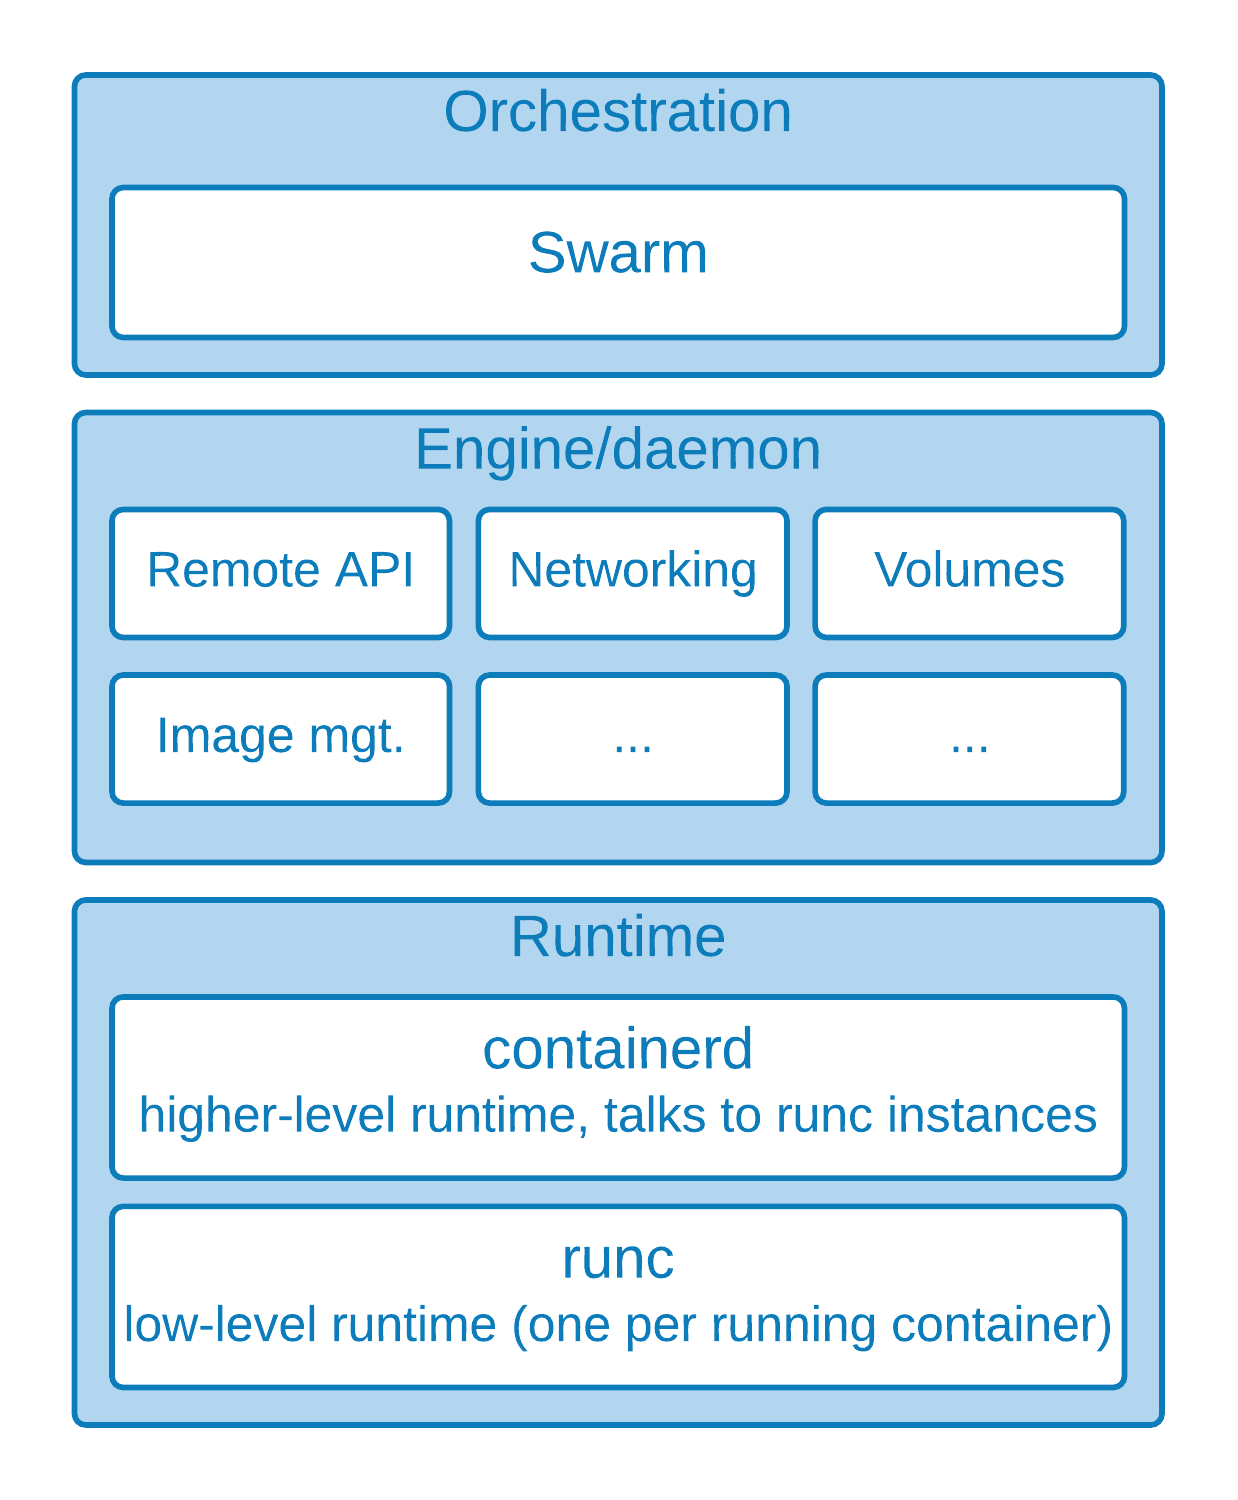
\includegraphics[width=0.5\columnwidth]{images/DockerArch.png}
    \caption{Docker Architektur \protect\cite{dockerdeep}}
    \label{fig:dockerarch}
\end{figure}

\section{Microservice}
\subsection{Aufbau}
\subsection{Entwicklung}
\subsection{Dezentrale Datenmanagement}


\section{Kubernetes}
\subsection{Architektur}
\subsection{Lightweight Kubernetes}
\subsection{Hybrid Cloud}
\subsection{Rancher}


%\subsubsection{Ein Unterabschnitt}

  % ... weitere Kapitel
 
  % Literaturverzeichnis
  \phantomsection
  \addcontentsline{toc}{chapter}{Literaturverzeichnis}
  \begin{thebibliography}{10}
    \bibitem{quelle1} Schreiberling, Tim: ,,Bestseller-Buch'', 1.~Auflage, S.~13ff, Renner-Verlag, Musterstadt, 2011.
  \end{thebibliography}
  \newpage
  
  % Anhang
  \phantomsection
  \addcontentsline{toc}{chapter}{Abbildungsverzeichnis}
  \listoffigures
  \newpage

  \phantomsection
  \addcontentsline{toc}{chapter}{Tabellenverzeichnis}
  \listoftables
  \newpage

  \phantomsection
  \addcontentsline{toc}{chapter}{Abkürzungsverzeichnis}
  \listoftables
  \newpage
  
  %\include{anhang}
\end{document}    